Following the study on the rejection of noise triggers using criteria presented in chapter \ref{section:selection} we will, in this chapter, further investigate why we have more single detector triggers on real data than on Gaussian noise.
Understanding why O3 single detector triggers have higher SNR could help in reducing their number or at least take actions to treat them adequately.
We will investigate one hypothesis in the present chapter: there may be excesses of noise on short time scales which cause fluctuations of the detector sensitivity that are not properly accounted for.

%%%%%%%%%%%%%%%%%% 

\subsection{Triggers boosted by fluctuations of the PSD}
\label{sec:triggers_PSD}

The detector sensitivity is directly related to its PSD and can be monitored using the local BNS range computed by the gating process (see section \ref{section:detection}).
This BNS range is computed over \SI{0.25}{s} at \SI{32}{Hz}, it has therefore fast variations.
Rather than this BNS range we will use the median range used for the gating, to monitor the sensitivity changes.
This median range is computed each second on the previous \SI{10}{s}.
We will call it \medr{}.

The reason we decide to use the to monitor the range fluctuations rather than the PSD itself is because the range allows to summarize the information given by the PSD in a single value.
Also the range is computed with the proper weight within the frequency band in which we expect to find astrophysical signals.
Noise at frequencies outside of this bandwidth will thus not make it fluctuate.

When doing the matched-filtering MBTA uses the median PSD over the last \SI{1000}{s} for the high frequency band and the last \SI{4000}{s} for the low frequency band.
% If we can show that the range at the time of the single detector triggers is in general lower than \SI{1000}{s} or \SI{4000}{s} before, then it could indicate a bias in the computation of the SNR.
We want to investigate how the \medr{} behaves close to the single detector triggers times and compare it to the median range computed over \SI{1000}{s} (range$_{1000s}$) or \SI{4000}{s} (range$_{4000s}$).
This may highlight some effect that could explain, at least in part, why we have more single detector triggers on real data than Gaussian noise.

%If an effect of some sort takes place we need to make sure it is actually something that causes background (bad) single detector triggers.
%In other words it should be an effect that is not seen when considering triggers of astrophysical origin nor should it be seen when looking at the gating range at random times.

\subsubsection{Range drop around triggers}

% O3
Figure \ref{fig:rangeO3} shows the distribution of the \medr{} at times where MBTA saved a background single detector trigger (i.e. excluding GWTC-2/3 triggers).
Only times which pass the single detector triggers criteria are considered.
We see that this distribution is shifted towards lower values when compared to the \medr{} distribution all over O3.
If this is due to extra noise at the time of the trigger, and not just due to the extra power coming from the event, we would be under-estimating the PSD and thus over-estimating the SNR of the triggers.
\begin{figure}[H]
  \centering
  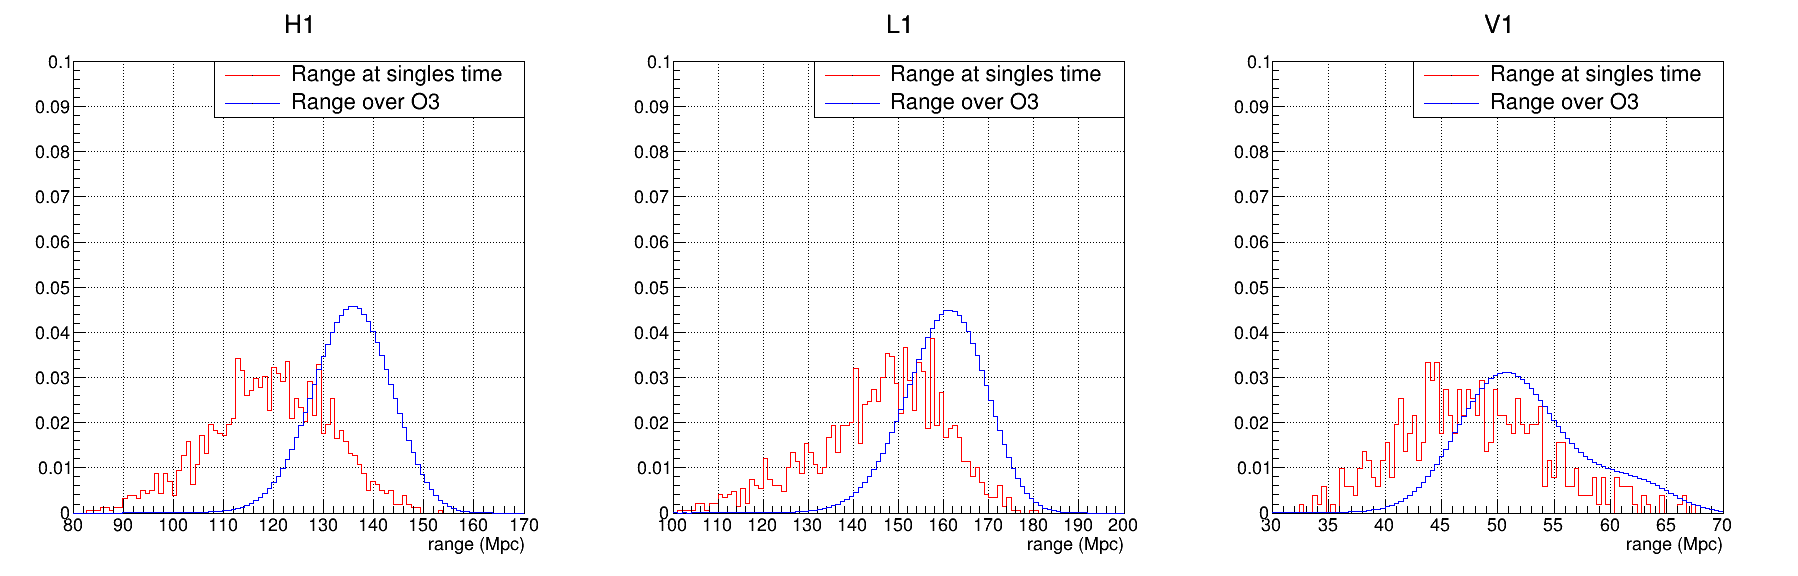
\includegraphics[width=\linewidth]{sectionBadTriggers/PSD/Range/range_ratio/cRangeO3_allCuts.png}
  \caption{\medr{} distribution over O3 (times which do not fit single selection criteria were removed).}
  \label{fig:rangeO3}
\end{figure}

Figure \ref{fig:rangeRatioO3} shows the distribution, for O3 background single detector triggers, of the \medr{} at the time of the single detector triggers compared to the range$_{1000s}$ and range$_{4000s}$.
We see that the \medr{} at the time of single detector trigger is indeed smaller compared to the median range computed on a longer time by more than 10\%.
\begin{figure}[H]
  \centering
  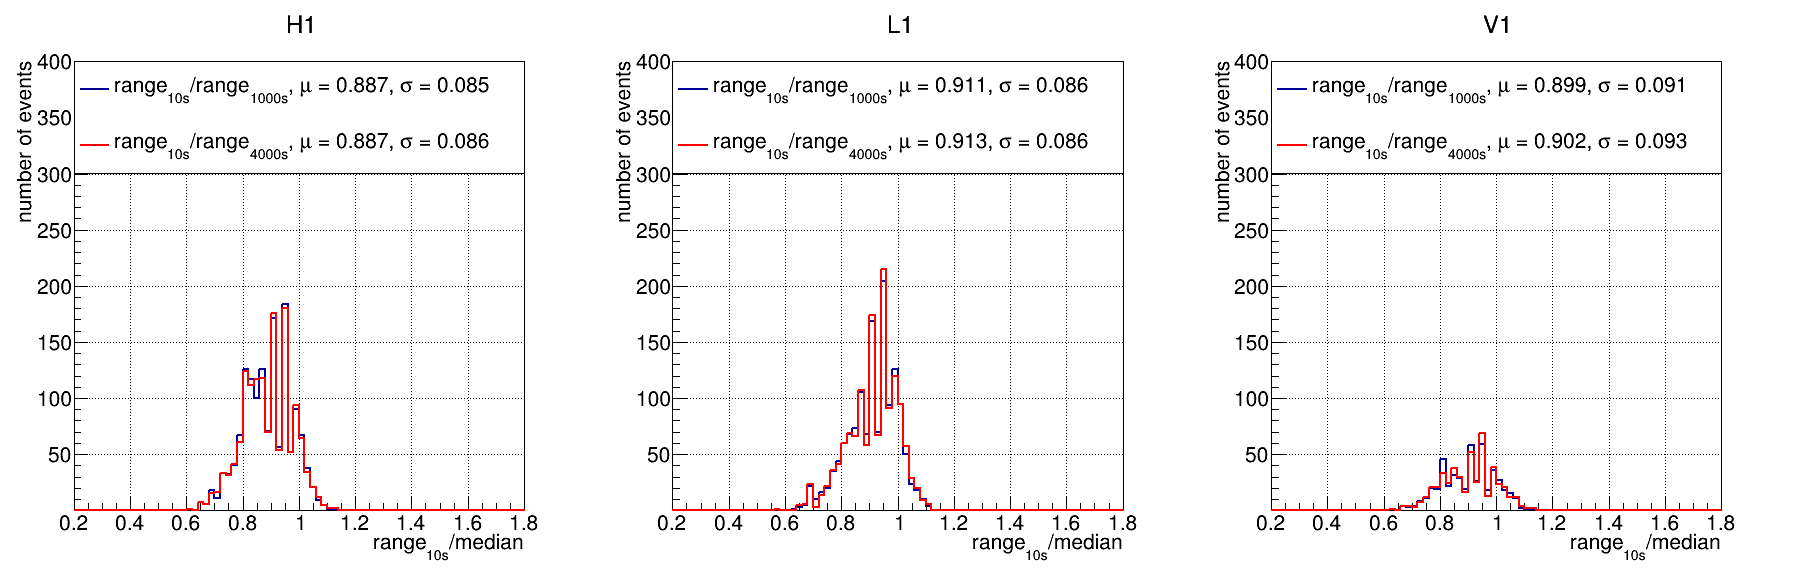
\includegraphics[width=\linewidth]{sectionBadTriggers/PSD/Range/range_ratio/cRatioMed_O3.png}
  \caption{\medr{}/range$_{1000(4000)s}$ for all of O3 singles (see text for the definition of the ratio).}
  \label{fig:rangeRatioO3}
\end{figure}

% EM bright singles
We wonder what the effect is on EM bright single detector triggers, as we have seen that we have less noise triggers for this population.
We see on figure \ref{fig:rangeRatioEMbright} that the effect is still present, although smaller ($\sim 1.7\text{-}2.9\% \pm \sim 0.4\%$) than when looking at all single detector tirggers.
\begin{figure}[H]
  \centering
  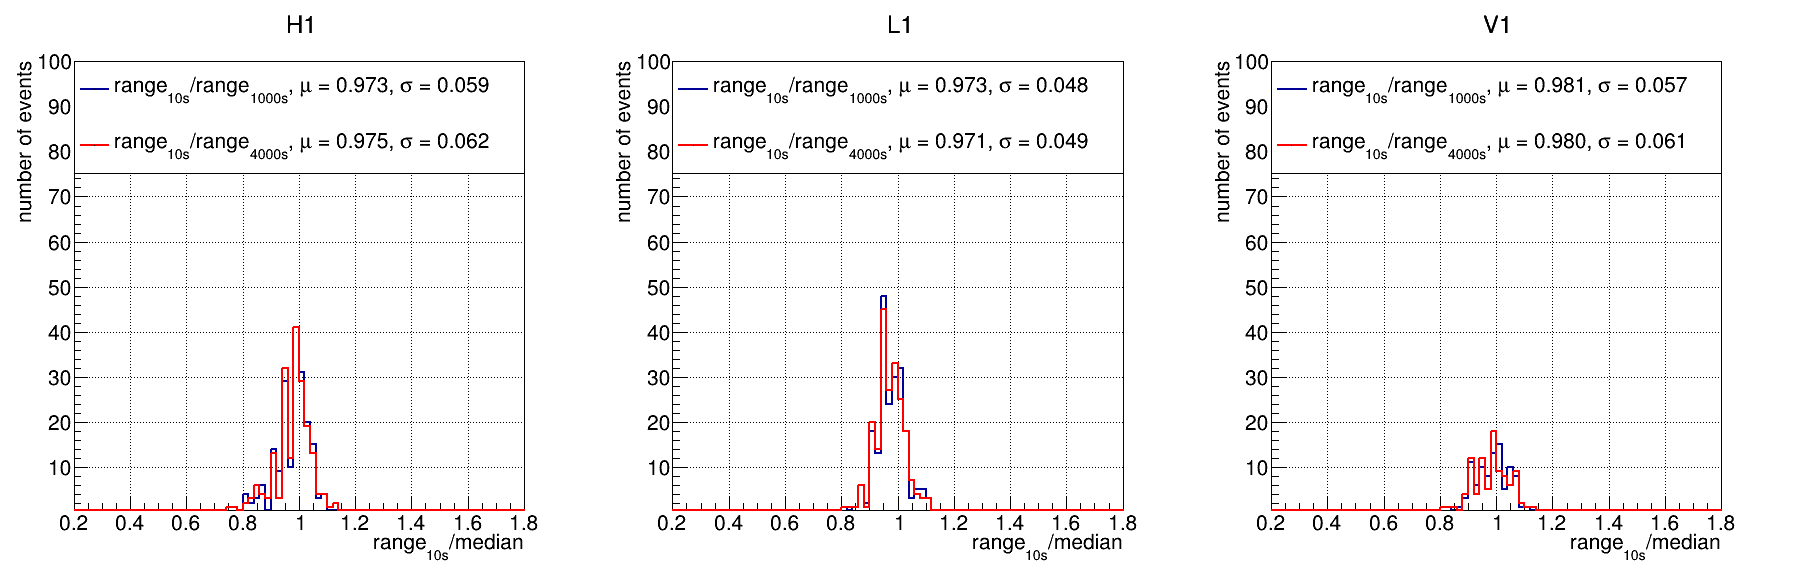
\includegraphics[width=\linewidth]{sectionBadTriggers/PSD/Range/range_ratio/cRatioMed_bright.png}
  \caption{\medr{}/range$_{1000(4000)s}$ for O3 EM bright singles with selection criteria applied. Their rwSNR distribution is shown in figure \ref{fig:compare_bright_gaus_selec}. Considering $\sim 200$ triggers in H1 or L1, the error on the mean value is $\sim 0.4\%$ in H1, $\sim 0.3\%$ in L1. For $\sim 100$ triggers in V1 the error on the mean value is $\sim 0.6\%$.}
  \label{fig:rangeRatioEMbright}
\end{figure}

Looking at O3 long EM dark single detector triggers after selection on ER and gating in figure \ref{fig:rangeRatioEMdarkLong}, we see that there is still a large offset of more than 10\%.
This is expected because although we called them ``long EM dark'' many of these triggers have a duration of only a few seconds.
An excess of power in the detector during a small duration will make the range drop on a short time.
\begin{figure}[H]
  \centering
  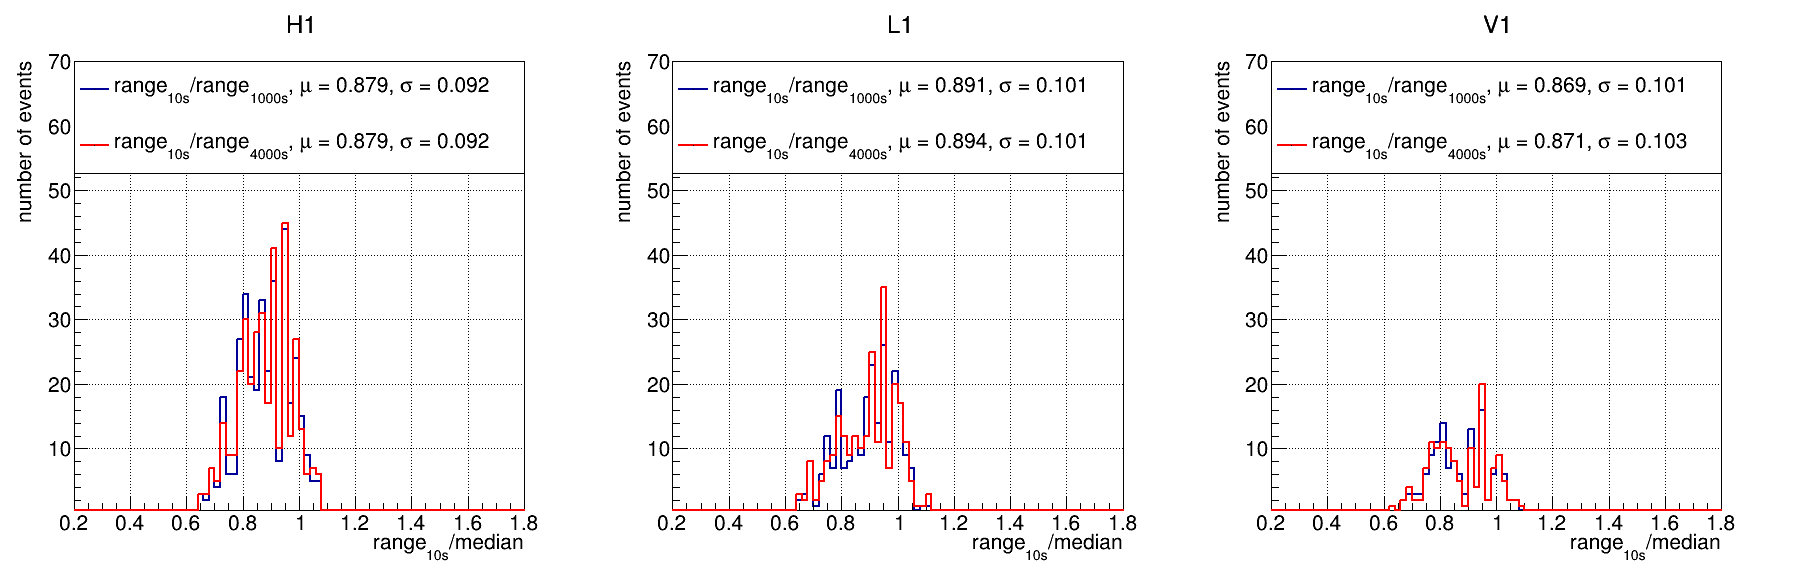
\includegraphics[width=\linewidth]{sectionBadTriggers/PSD/Range/range_ratio/cRatioMed_darkLong.png}
  \caption{\medr{}/range$_{1000(4000)s}$ for O3 long EM dark singles with selection criteria applied.}
  \label{fig:rangeRatioEMdarkLong}
\end{figure}

% Gaussian noise
We can also check whether this effect occurs for Gaussian noise, as it consists of low SNR triggers.
The range computed on Gaussian noise should not fluctuate a lot.
Thus, we expect the effect to be much smaller, if there is an effect.
Figure \ref{fig:rangeRatioGaus} shows the distribution of the range ratio for single detector triggers obtained on Gaussian noise.
We see that we have here an effect smaller than 1\%.
\begin{figure}[H]
  \centering
  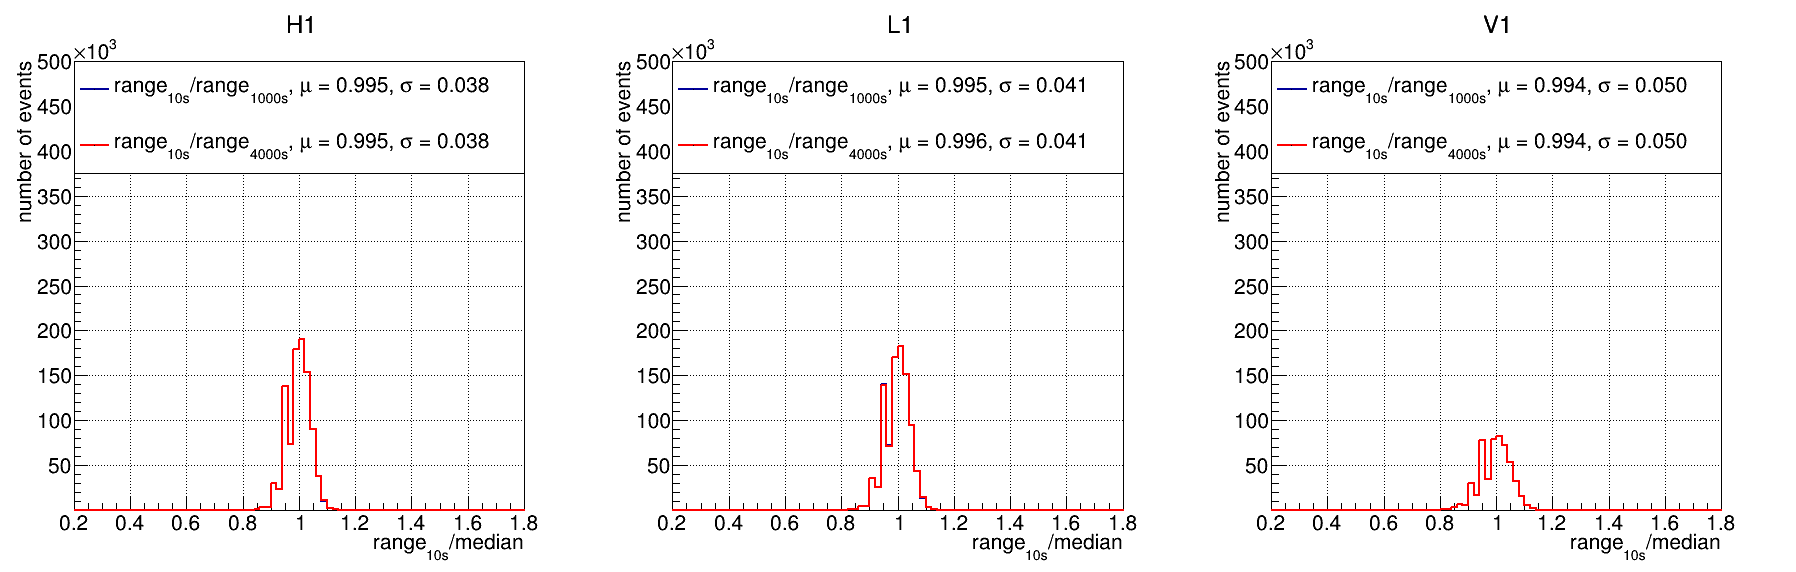
\includegraphics[width=\linewidth]{sectionBadTriggers/PSD/Range/range_ratio/cRatioMed_Gaus.png}
  \caption{\medr{}/range$_{1000(4000)s}$ for all (EM bright or not) single detector triggers obtained from a Gaussian noise analysis. The distribution is rescaled to O3 observing time.}
  \label{fig:rangeRatioGaus}
\end{figure}

The EM bright single detector triggers which passed the selection criteria defined in section \ref{section:selection} were compared to triggers obtained on Gaussian noise in figure \ref{fig:compare_bright_gaus_selec}.
Taking the mean value of the histograms in figures \ref{fig:rangeRatioEMbright}, we can shift this Gaussian noise by 2.6\% in H1 and 2.9\% in L1.
Figure \ref{fig:shiftGausBright} shows the comparison of the shifted Gaussian noise distribution with the single detector triggers.
We see that we can explain part of the difference between the two with the observed effect.
However, this shift of the Gaussian noise assumes that all the range reduction observed at the time of single detector triggers is coming from extra noise.
We have to see if this is a background-only effect.
One way to investigate this, is to have a look at astrophysical signals and randomly selected times.
\begin{figure}[H]
  \centering
  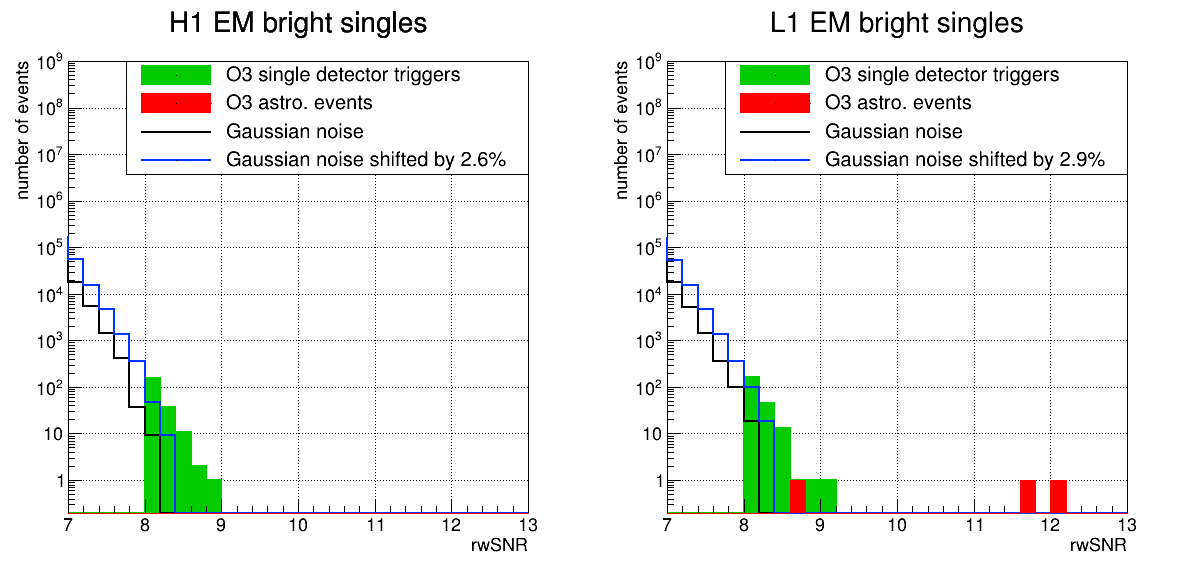
\includegraphics[width=\linewidth]{sectionBadTriggers/PSD/Reweight/cBrightGausShift.png}
  \caption{Comparison of O3 EM bright single detector triggers which passed the selection to shifted Gaussian noise distributions using the observations described in this section.}
  \label{fig:shiftGausBright}
\end{figure}

\subsubsection{Range drop due to astrophysical signals}

% astro
Astrophysical signals could also reduce the ``local'' range because they are adding signal on top of the detector noise.
Therefore they can increase the PSD of the detector.
In this section, we are investigating this effect, to see if it explains all or only part of the observed range change described in the previous section.

Figure \ref{fig:rangeRatioAstro} shows the same distributions as figure \ref{fig:rangeRatioO3} for single detector triggers associated to O3 astrophysical events (all type mixed, selection criteria applied).
We see that the effect is indeed present but not as strong as in figure \ref{fig:rangeRatioO3}, however there is only a small number of detection which prevents us to draw any solid conclusion.
%
\begin{figure}[H]
  \centering
  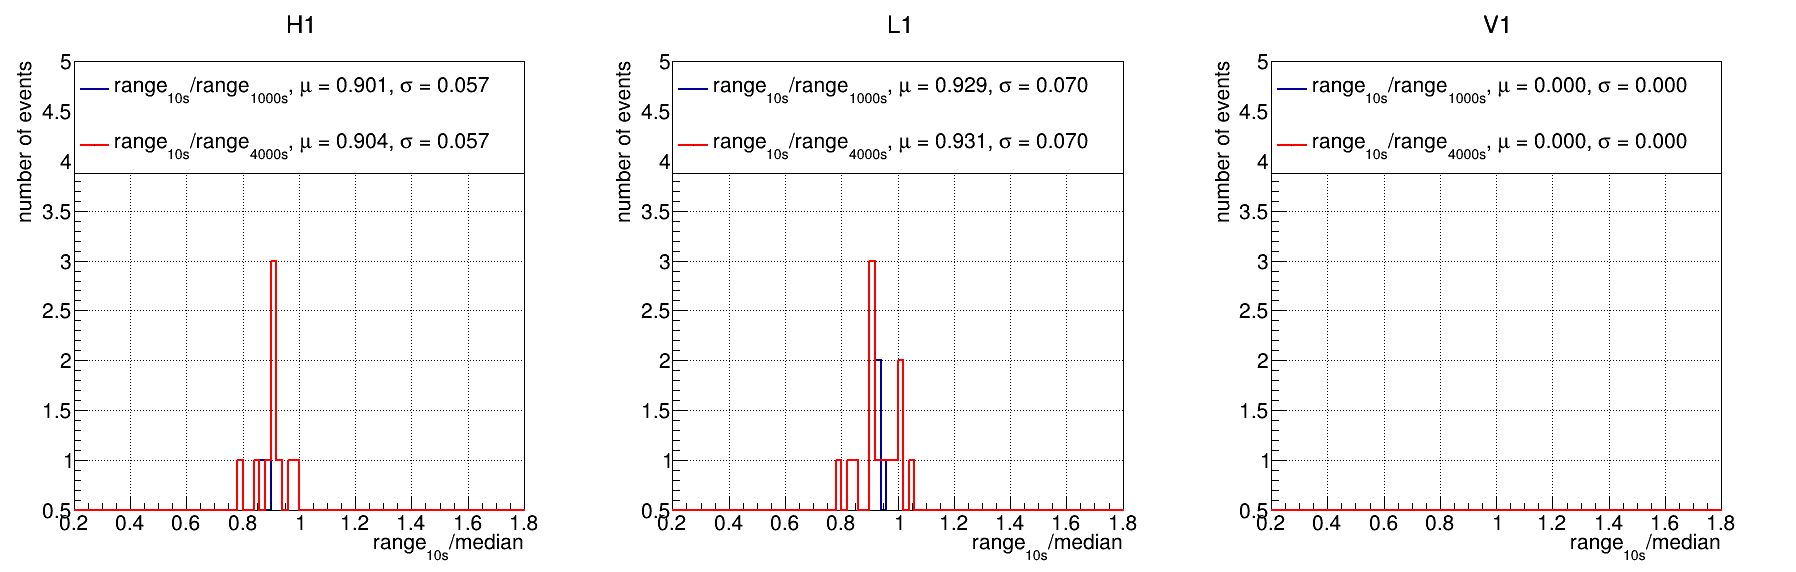
\includegraphics[width=\linewidth]{sectionBadTriggers/PSD/Range/range_ratio/cRatioMed_astro.png}
  \caption{\medr{}/range$_{1000(4000)s}$ for all O3 astrophysical triggers.}
  \label{fig:rangeRatioAstro}
\end{figure}

% MDC
To overcome the low statistics issue, we can also see this effect for simulated astrophysical signal as shown in figure \ref{fig:rangeRatioMDC} for injections on O3 data, analyzed with the O4 configuration of the pipeline.
They are split in EM bright and EM dark populations.
The effect is smaller for the EM bright injections, with a shift smaller than 1\% in the distribution.
This is for the same reason as O3 single detector triggers.
BBH injections are loud and short, causing a drop in the range of the detector.
On the other hand, for EM dark injections, the effect is of the same order of magnitude as for real astrophysical signals: $\sim$ 7.1-9.3\%.
Comparing the offset for O3 EM bright single detector triggers ($\sim 1.7\text{-}2.9\% \pm \sim 0.4\%$) with the offset for EM bright injections ($\sim 0.5\text{-}0.8\% \pm \sim 0.1\%$), the effet is statistically significant.
%
\begin{figure}
  \centering
  \begin{minipage}{\linewidth}
    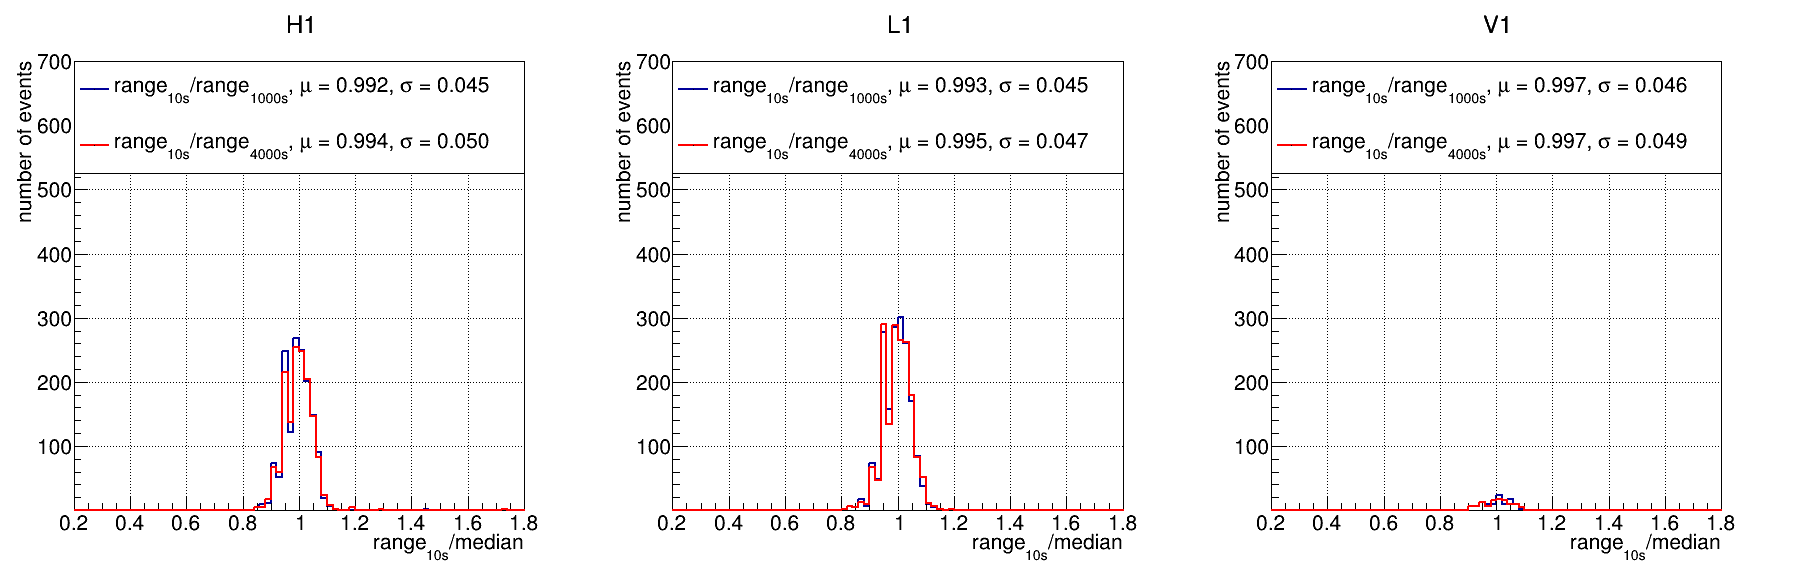
\includegraphics[width=\linewidth]{sectionBadTriggers/PSD/Range/range_ratio/cRatioMed_injMDC_bright.png}
  \end{minipage}
  %
  \begin{minipage}{\linewidth}
    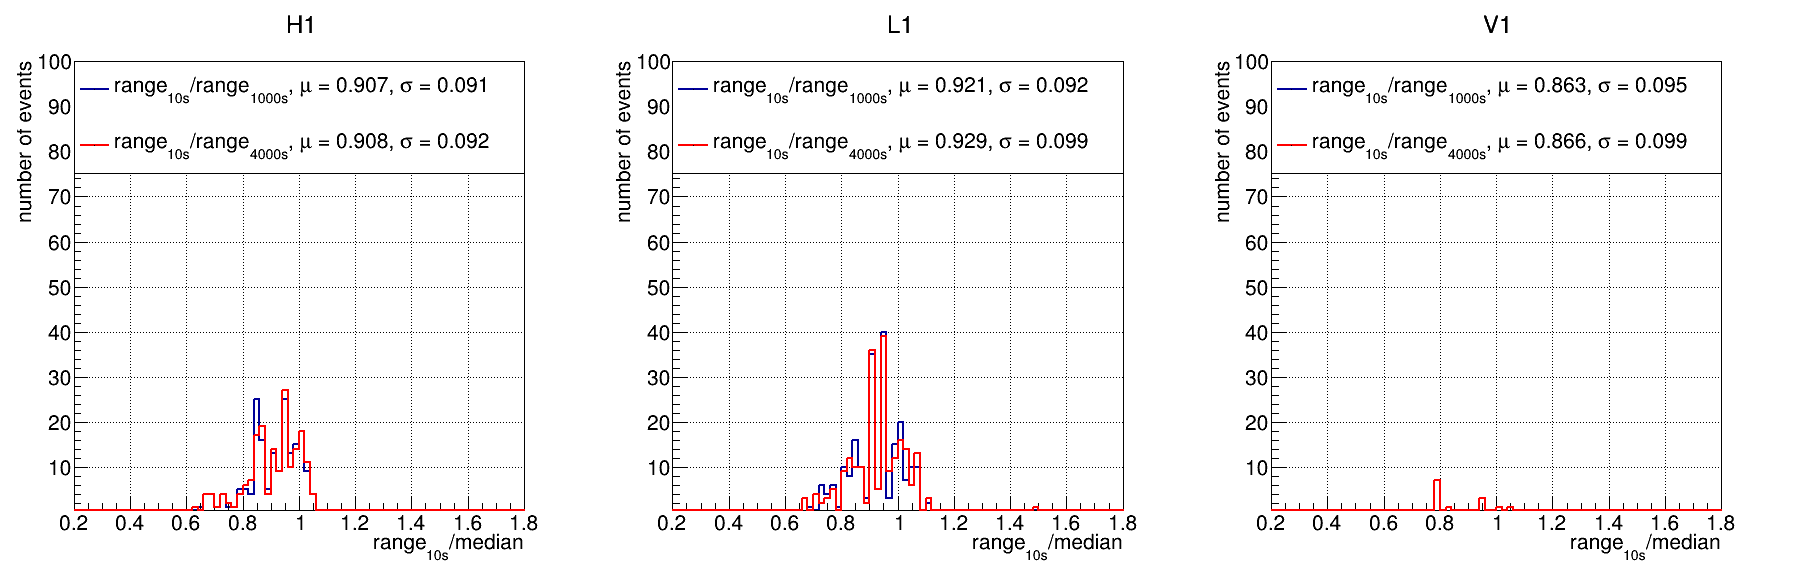
\includegraphics[width=\linewidth]{sectionBadTriggers/PSD/Range/range_ratio/cRatioMed_injMDC_dark.png}
  \end{minipage}
  \caption{\medr{}/range$_{1000(4000)s}$ for recovered injections added to O3 data, analyzed using MBTA O4 configuration. Top: EM bright population. Bottom: EM dark population.
  For EM bright injections, considering $\sim 1500$ recovered injections in H1 and $\sim 1750$ in L1 the error on the mean is $\sim 0.1\%$ for both. It is $\sim 0.4\%$ in V1 due to fewer recovered injections.}
  \label{fig:rangeRatioMDC}
\end{figure}

% random times
On the contrary, we do not expect to see such an effect if we look at the variation of the \medr{} at random times.
This is confirmed by figure \ref{fig:rangeRatioRandomTimes} which shows a deviation smaller than $0.3\%$.
\begin{figure}[H]
  \centering
  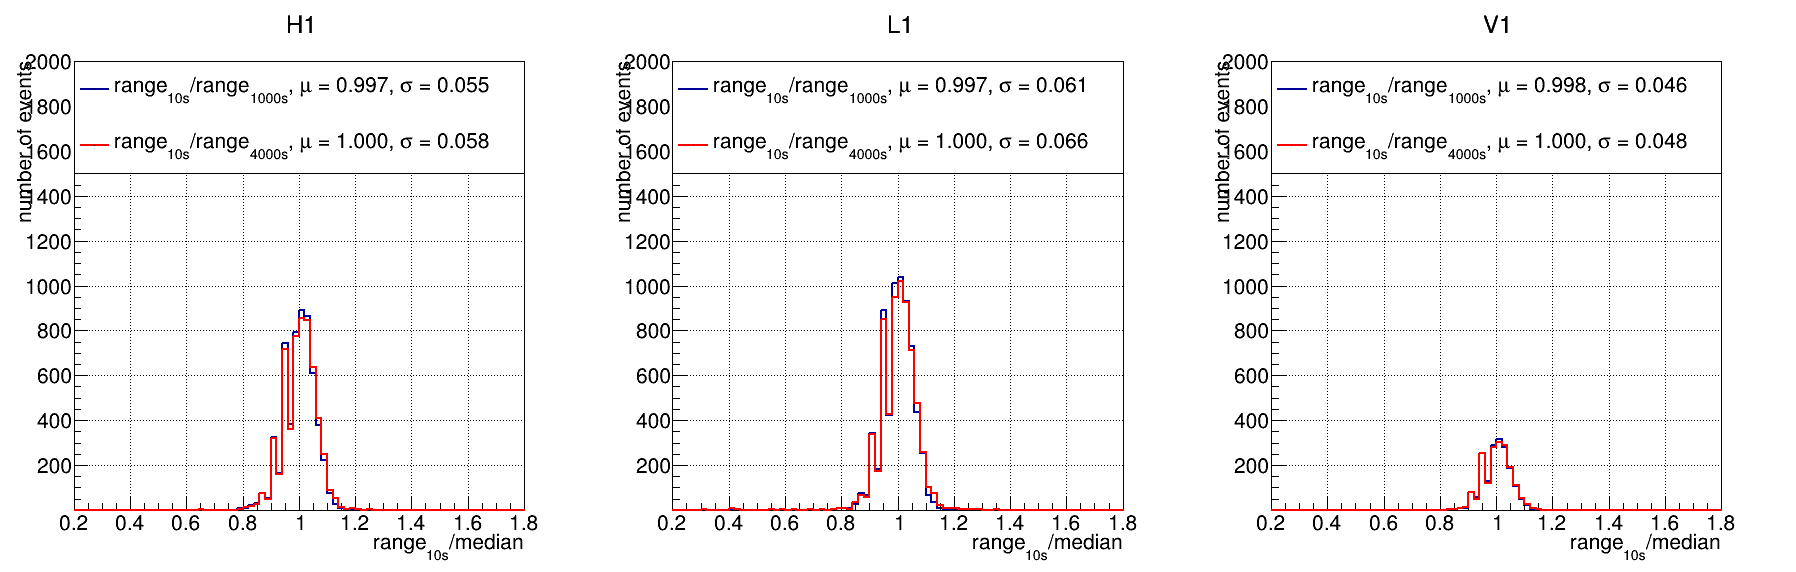
\includegraphics[width=\linewidth]{sectionBadTriggers/PSD/Range/range_ratio/cRatioMed_switchDet.png}
  \caption{\medr{}/range$_{1000(4000)s}$ for random times.}
  \label{fig:rangeRatioRandomTimes}
\end{figure}

This is strong evidence in favour of our initial hypothesis: there are PSD fluctuations that are not properly accounted for when performing the matched-filtering, causing the PSD to be under-estimated at trigger times leading to over-estimate their SNR values.
This results in a larger number of single detector triggers above a given SNR threshold.

\subsubsection{Time scale of the drop in range}

We want to know on what time scale the drop in sensitivity happens.
Starting with all background single detector triggers, we compute for all of them the ratio of the range at each time with the \medr{} at the time of the trigger.
Then, at each time, we take the median value of the ratio over all EM bright single detector triggers.
The black curve in figure \ref{fig:rangeOverTime} shows the evolution over time of the median of the ratio over all EM bright triggers.
We see that the time scale and magnitude of the effect depends on the detector, with L1 being the one in which it is the most visible.
It also appears that the minimum for the ratio is reached just a few seconds before the trigger.

We have seen that there is no offset for random times.
But we can create one by selecting cleverly our random times (which are therefore not so random anymore).
We can search, for each random time, the time which has the minimum \medr{} value within for example $\pm$ \SI{40}{s}.
If we then compute the range ratio around this time, we should see a similar effect to the one observed for single detector triggers.
This is shown by the red curve in figure \ref{fig:rangeOverTime}.
We see that the drop in the ratio is much larger than what is observed for single detector triggers.
But unlike the effect observed in L1, the drop happens only in a matter of seconds corresponding to the time window on which the local \medr{} is computed.
%
\begin{figure}[H]
  \centering
  \begin{minipage}{\linewidth}
    \centering
    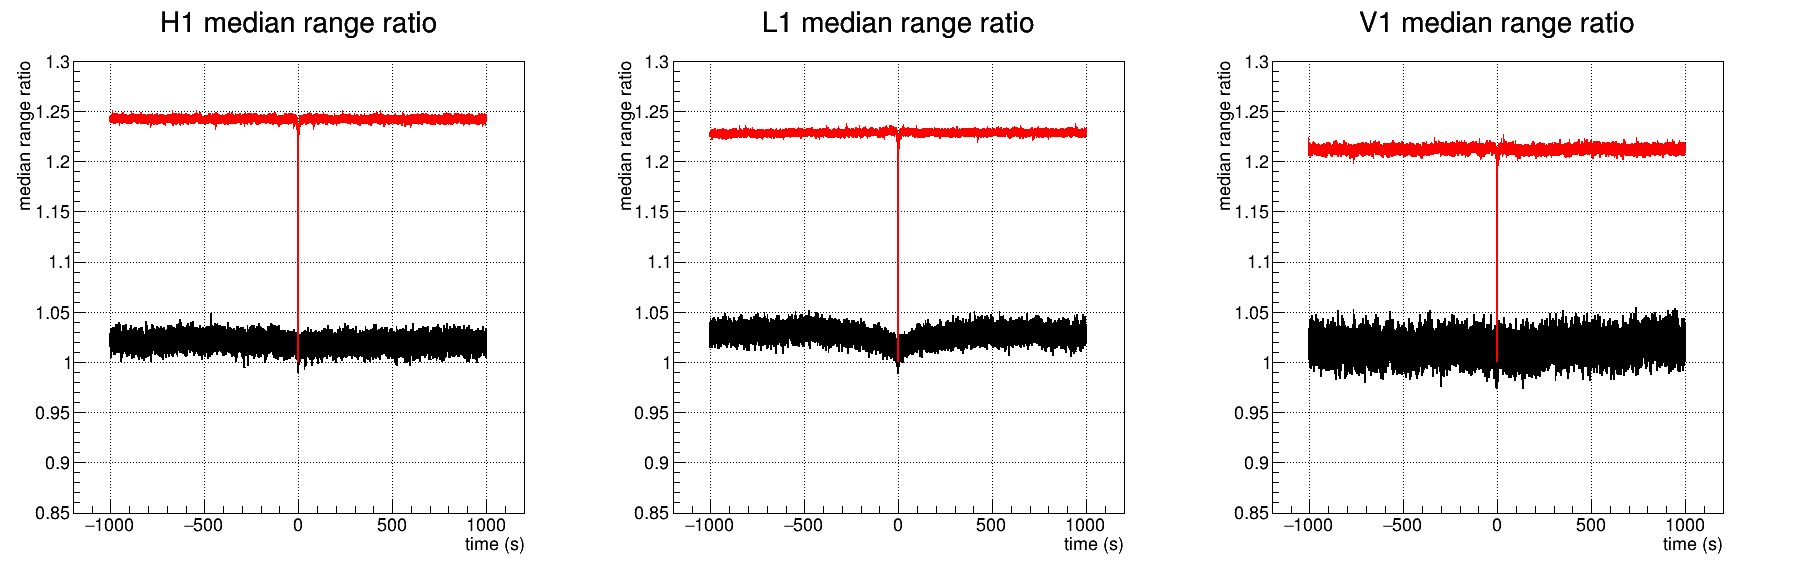
\includegraphics[width=\linewidth]{sectionBadTriggers/PSD/Range/range_ratio/cAroundCompare.png}
  \end{minipage}
  % 
  \begin{minipage}{\linewidth}
    \centering
    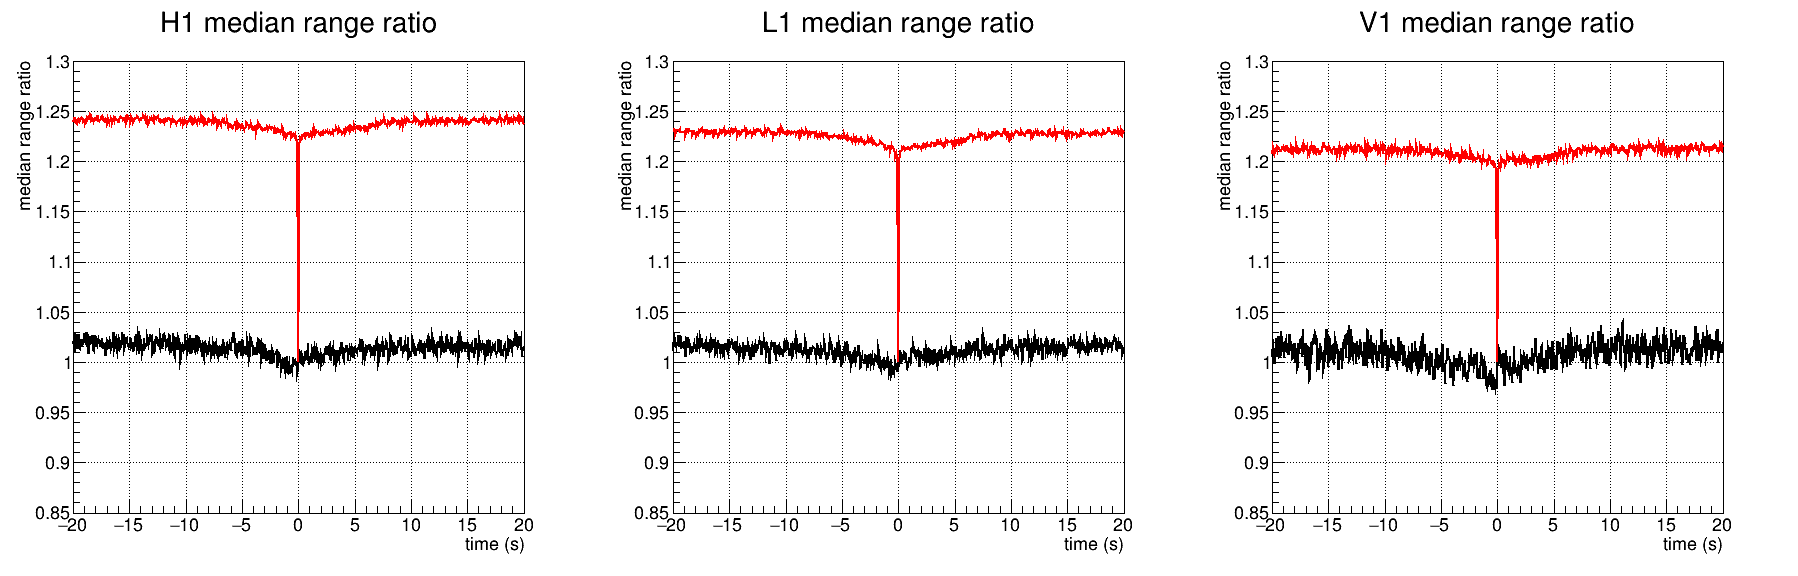
\includegraphics[width=\linewidth]{sectionBadTriggers/PSD/Range/range_ratio/cAroundCompare_zoom.png}
  \end{minipage}
  \caption{range(t)/range(t$_0$=0) (t$_0$ being the time of the single detector trigger or minimum range for random times). The figure is showing in black for each bin the median value over all EM bright single detector triggers. The red line shows the same for the lowest value of random segments (see text). Top: looking at $\left[-1000; +1000\right]$ s. Bottom: zoom on $\left[-20; +20\right]$ s}
  \label{fig:rangeOverTime}
\end{figure}




%%%%%%%% reweighting
\clearpage
\subsection{Correcting the SNR for range fluctuations}
\label{sec:correc_snr_range}

Solving the issue highlighted in the previous section is no easy task.
The PSD can't be measured with precision on short durations with high frequency resolution.
Instead an idea was to apply a correction to the SNR by taking into account the range fluctuations around the time of the trigger.
The weight applied would be the ratio between the \medr{} at the time of the single detector trigger and the median range computed over a "much longer" duration before the trigger.
It would also mean reducing the SNR of astrophysical signals.
For instance, the 3 EM bright astrophysical events of O3, GW190425, GW200105\_162426 and GW200115\_042309 have a range ratio of 0.99, 0.97 and 1.00.
But we can still have a look at the effect of the correction for background tirggers.

Figure \ref{fig:reweightBrightInstant} shows the comparison of the uncorrected distribution with the distribution corrected using the range ratios \medr{}/range$_{1000s}$.
Two types of corrections are shown: considering all range ratios (meaning that the SNR can be increased by the correction) and considering only ratios smaller than 1.
We see that, considering all ratios, even if we have less single detector triggers above rwSNR=8 overall, the result is not satisfactory as we now have more triggers with SNR around 9.
Using only ratios smaller than 1, however, allow to reduce nicely the background.
We will therefore only consider corrections when the range ratio is smaller than 1 in the following.

Accounting for the time scale of the range drop as shown in figure \ref{fig:rangeOverTime}, we decide to investigate a correction using a median value of the \medr{} instead of the instantaneous value at the time of the trigger.
This should avoid to be sensible to the rapid fluctuations of the range ratio.
The result is shown in figure \ref{fig:reweightBright_b}.
The correction here is done using the median value of the \medr{} over the \SI{4}{s} preceding the triggers (chosen arbitrarily), divided by range$_{1000s}$.
It is compared to the correction using the \medr{} at the time of the event.
It makes things slightly better at high rwSNR.

Additionnally, we may wonder how important the choice of \SI{4}{s} was for the computation of the median.
Figure \ref{fig:reweightBright} shows that the duration chosen for the computation indeed has an impact on the result, but it is not clear what the best choice is.
Note that we have only considered range ratios smaller than 1 here.
The range$_{1000s}$ was chosen for this figure.
\begin{figure}[H]
  \centering
  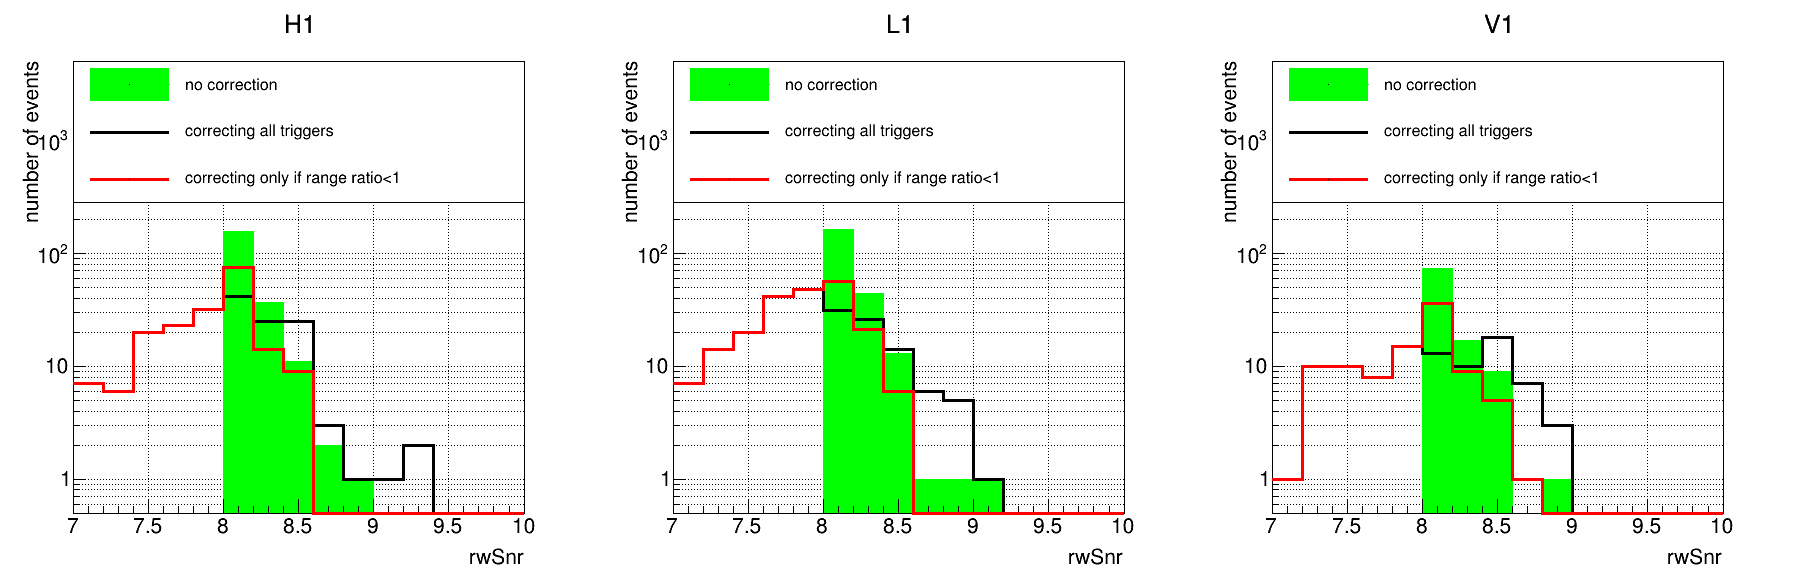
\includegraphics[width=\linewidth]{sectionBadTriggers/PSD/Reweight/cThese1_bright.png}
  \caption{Corrected distribution compared to the original distribution for O3 EM bright singles (with selection criteria) using \medr{}/range$_{1000s}$. Black: correcting all triggers. Red: correcting only if the ratio is smaller than one.}
  \label{fig:reweightBrightInstant}
\end{figure}
%
\begin{figure}[H]
  \centering
  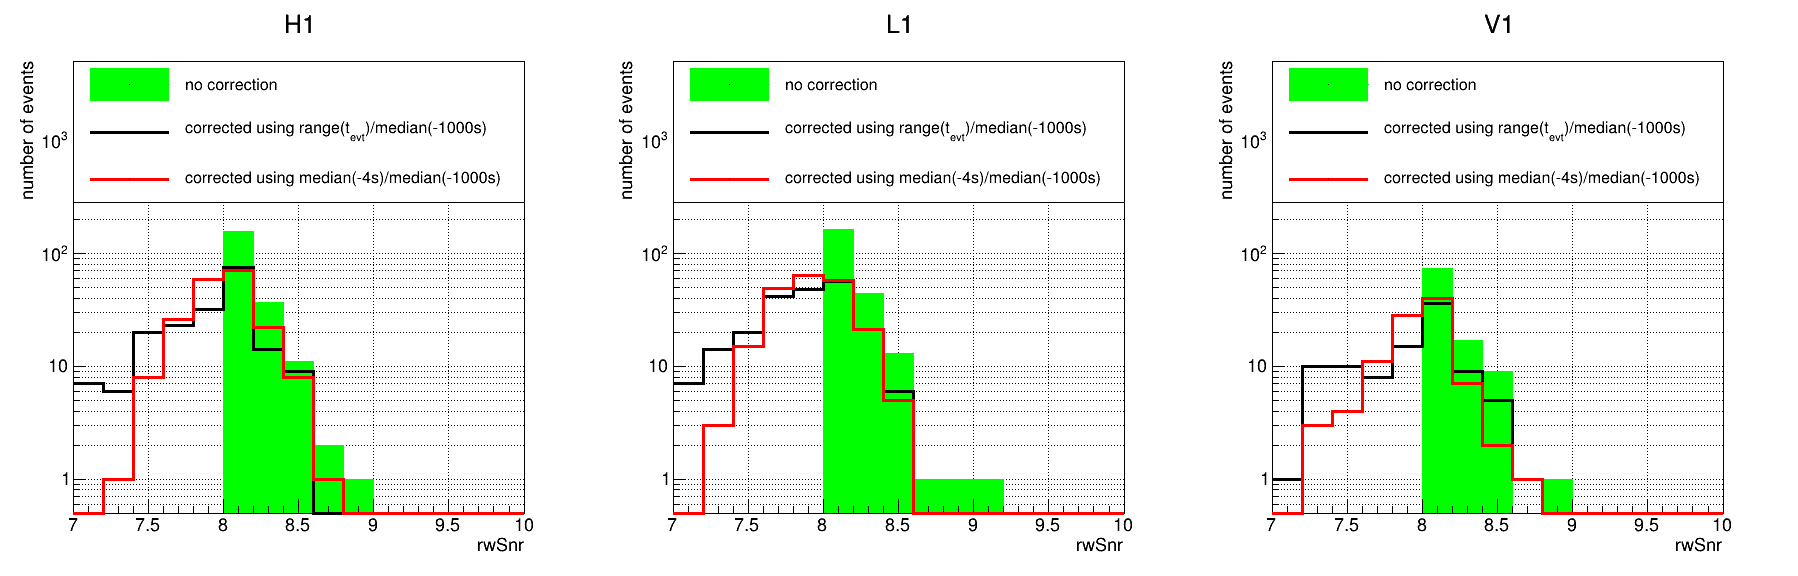
\includegraphics[width=\linewidth]{sectionBadTriggers/PSD/Reweight/cThese2_bright.png}
  \caption{Corrected distribution for O3 EM bright singles (with selection criteria). Black: \medr{}/range$_{1000s}$. Red: using the median over \SI{4}{s} before the trigger of the \medr{} instead of the medan range. Corrections are only applied if the ratio is smaller than one.}
  \label{fig:reweightBright_b}
\end{figure}
%
\begin{figure}[H]
  \centering
  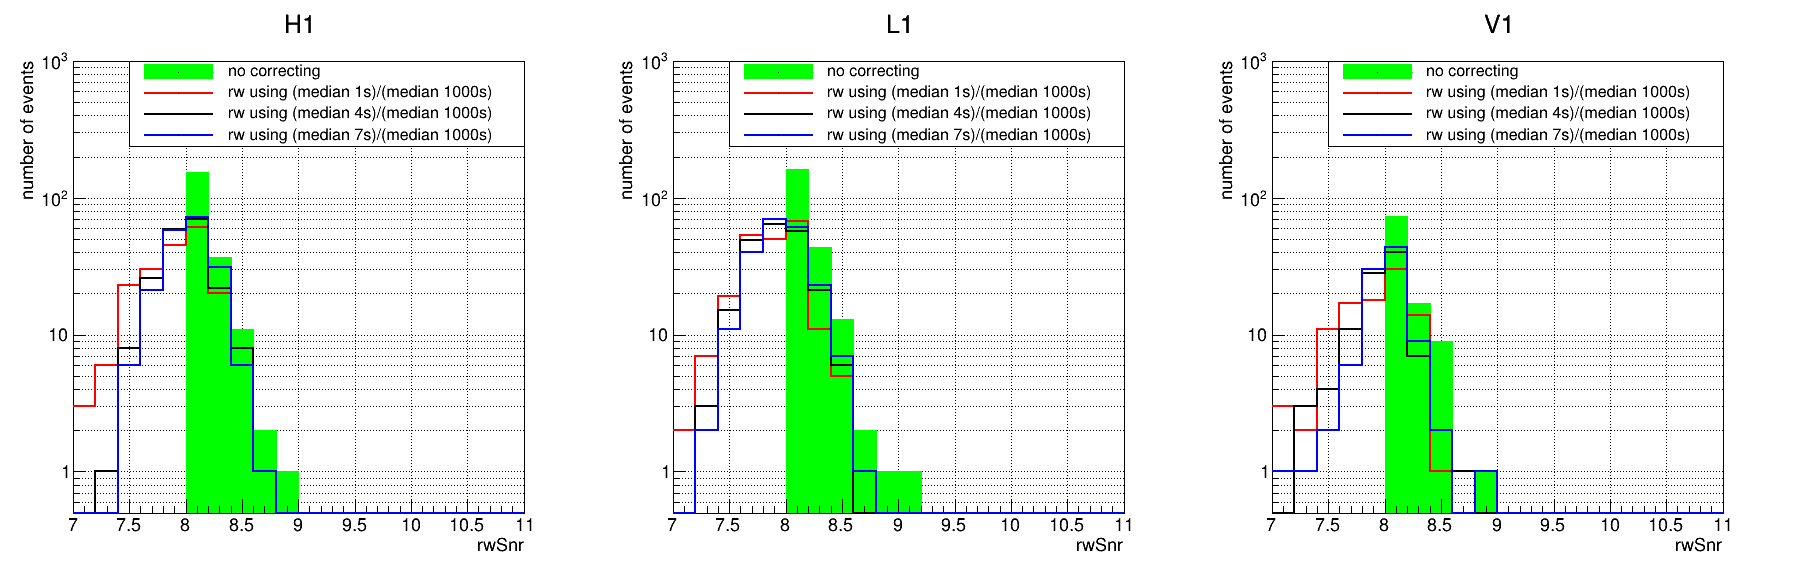
\includegraphics[width=\linewidth]{sectionBadTriggers/PSD/Reweight/cReweightBright.png}
  \caption{Corrected distribution compared to the original distribution for EM bright singles using various median values of the \medr{} before the trigger. Corrections are only applied if the ratio is smaller than one.}
  \label{fig:reweightBright}
\end{figure}

We saw earlier that shifting the Gaussian noise rwSNR distribution by a few percent (according to the previous section) reduced the difference between O3 EM bright single detector triggers and the Gaussian noise distribution.
We now try another approach and investigate if correcting the SNR using the range ratio affects the single detector triggers obtained on Gaussian noise.
Figure \ref{fig:reweightGaus} shows that the Gaussian noise is barely affected by this reweighting.
Figure \ref{fig:reweightBrightGaus} shows the comparison of the corrected distribution for O3 EM bright single detector triggers with the corrected distribution for the Gaussian noise.
The two distribution are now indeed closer to one another, although there is still room for improvement.
\begin{figure}[H]
  \centering
  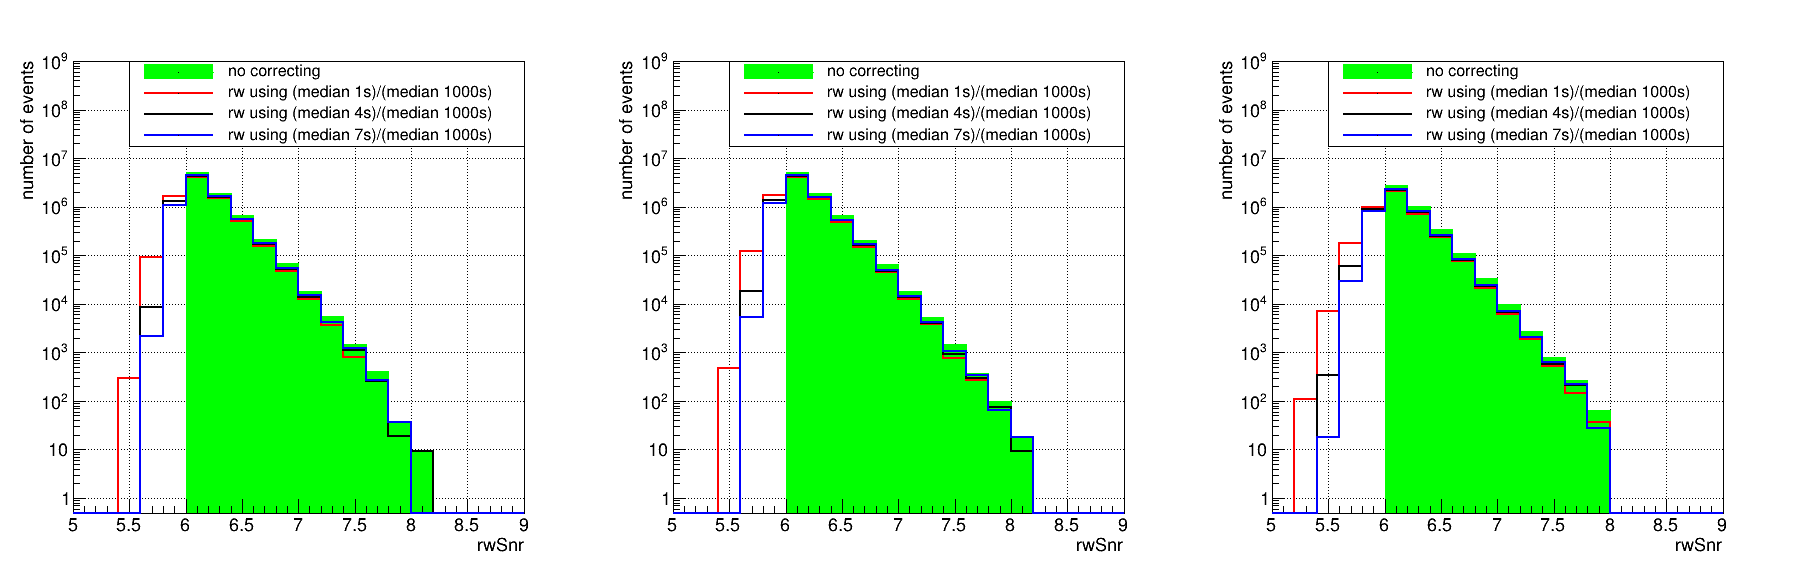
\includegraphics[width=\linewidth]{sectionBadTriggers/PSD/Reweight/cReweightGausBright.png}
  \caption{Corrected distribution for the EM bright single detector triggers obtained by analyzing the same gaussian noise as in section \ref{section:selection}. Note that the Gaussian noise distribution is scaled to the observing time of O3. Corrections are only applied if the ratio is smaller than one.}
  \label{fig:reweightGaus}
\end{figure}
%
\begin{figure}[H]
  \centering
  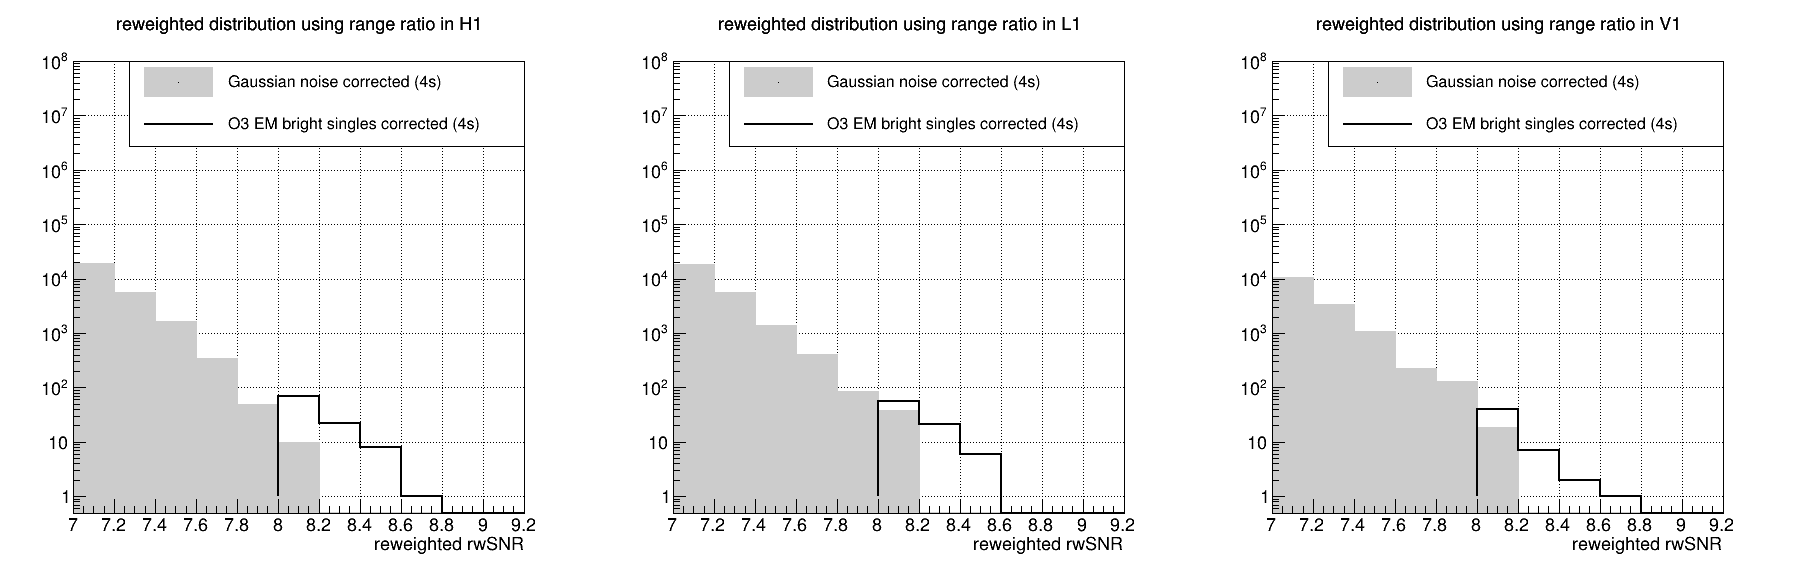
\includegraphics[width=\linewidth]{sectionBadTriggers/PSD/Reweight/cReweightBrightGaus.png}
  \caption{Corrected O3 EM bright single detector triggers distribution compared to the corrected gaussian noise distribution (also EM bright singles, scaled to O3 observing time). The correction is the ratio of the median computed over \SI{4}{s} before the trigger with the range$_{1000s}$. Corrections are only applied if the ratio is smaller than one. O3 events with a corrected rwSNR smaller than 8 (initial selection threshold) were not included in this figure.}
  \label{fig:reweightBrightGaus}
\end{figure}

We can also investigate a correction for the long EM dark single detector triggers.
We saw that for injections, the mean value of the range ratio distribution was smaller than 1, for instance 0.92 in L1.
In order to correct the SNR of the single detector triggers without impacting too much the injections, we choose to correct the SNR if the range ratio is smaller than 0.92.
Figure \ref{fig:reweightDarkInstant} shows the effect of the correction when considering all long EM dark single detector triggers and when considering only those with ratio smaller than 0.92.
We want the correction we apply to start at 1 when the ratio is 0.92 and decrease for lower values.
The correction applied is therefore the ratio divided by 0.92.
Figure \ref{fig:reweightDark_b} show the effect of the correction (for range ratios smaller than 0.92) on O3 long EM dark single detector triggers when considering the median of the \medr{} over the \SI{4}{s} preceding the trigger in the ratio.
We see that for long EM dark triggers, using the \medr{} at the time of the trigger allows to reject more triggers while using the median over \SI{4}{s} has almost no impact.
This is explained by the fact that the drop in the range for long EM dark triggers happens in a short time and is more important than for EM bright single detector triggers.
Therefore taking the median value of the \medr{} over the \SI{4}{s} before the tirgger makes the difference with the range$_{1000s}$ before the tirgger much smaller.
Since we chose to correct triggers with a ratio smaller than 0.92, only a very small number of triggers are corrected in this case.
\begin{figure}[H]
  \centering
  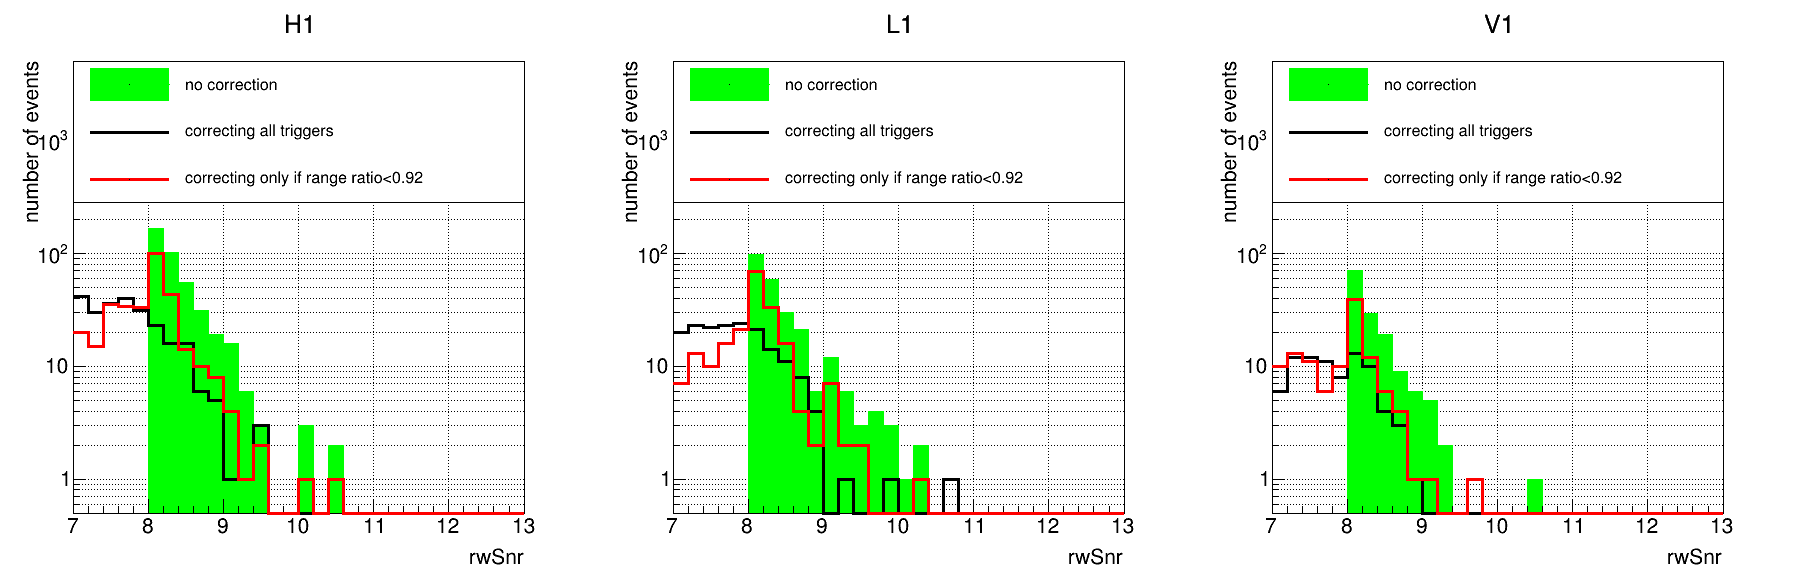
\includegraphics[width=\linewidth]{sectionBadTriggers/PSD/Reweight/cThese1_darkLong.png}
  \caption{Corrected distribution compared to the original distribution for O3 long EM dark singles (with selection criteria) using \medr{}/range$_{1000s}$. Black: correcting all triggers. Red: correcting only if the ratio is smaller than 0.92.}
  \label{fig:reweightDarkInstant}
\end{figure}
%
\begin{figure}[H]
  \centering
  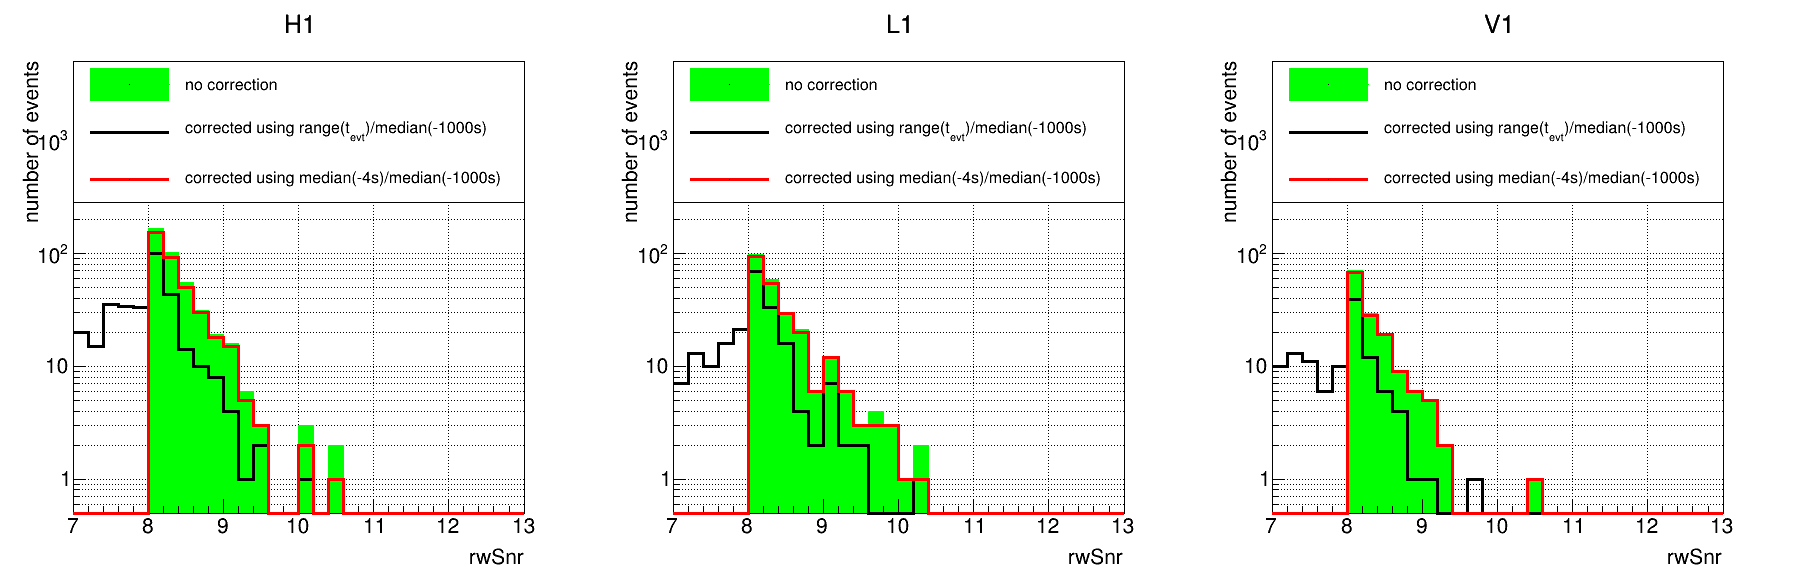
\includegraphics[width=\linewidth]{sectionBadTriggers/PSD/Reweight/cThese2_darkLong.png}
  \caption{Corrected distribution for O3 long EM dark singles (with selection criteria). Black: using \medr{}/range$_{1000s}$. Red: using the median over \SI{4}{s} before the trigger of the \medr{}. Corrections are only applied if the ratio is smaller than 0.92 and is equal to the ratio divided by 0.92.}
  \label{fig:reweightDark_b}
\end{figure}

It was decided to leave things as they were for O4.
The understanding we acquired of this mechanism tells us that this effect is taken into account in the method we use to compute the background for the FAR of the single detector triggers, presented in chapter \ref{section:far}.





%%%%%%%%%%%%%%%%%%%%%%%%%%%%%%%%%%%%%%%%%%%%%%%%%%%%%% 
%%%%%%%%%%%%%%%%%%%%%%%%%%%%%%%%%%%%%%%%%%%%%%%%%%%%%% 


% \begin{figure}[H]
%   \centering
%   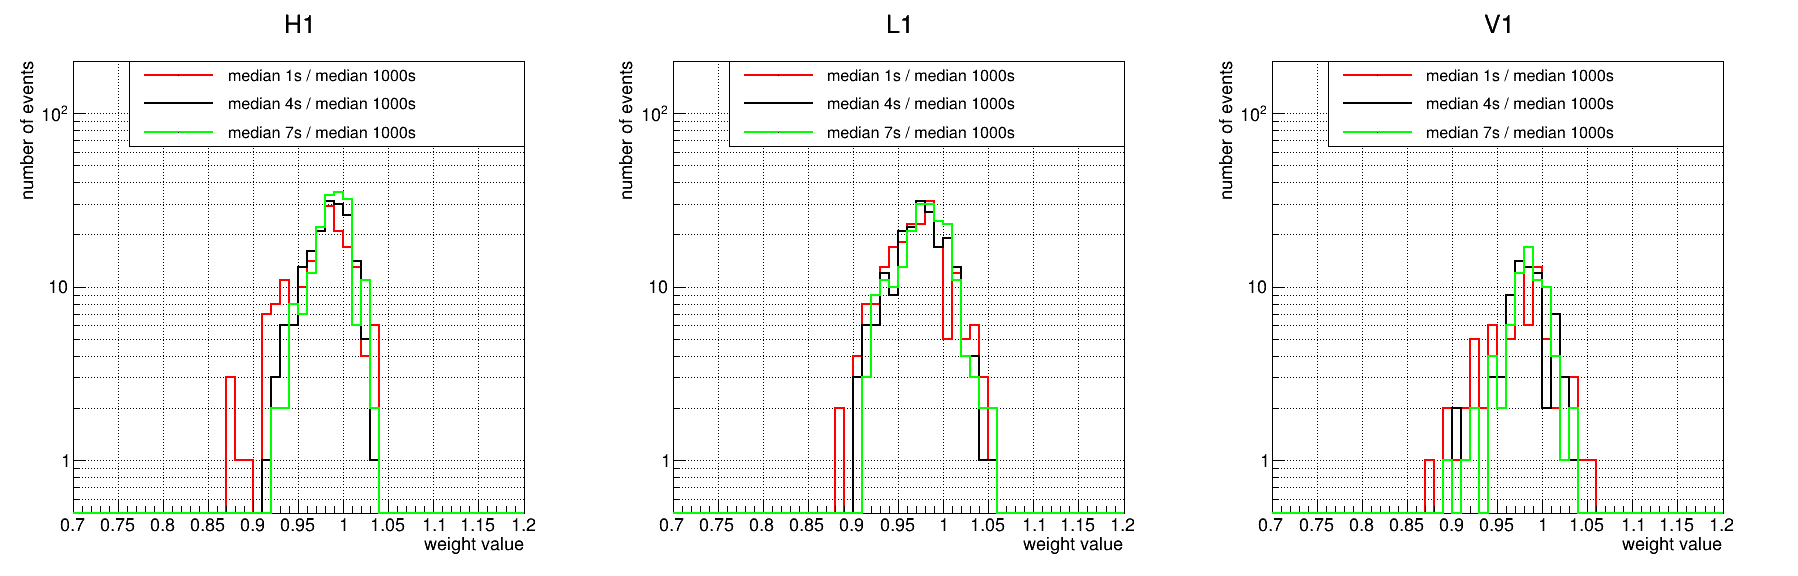
\includegraphics[width=\linewidth]{sectionBadTriggers/PSD/Reweight/cWeightBright.png}
%   \caption{Correction weights distribution for EM bright singles}
%   \label{fig:weightBright}
% \end{figure}

% \begin{figure}[H]
%   \centering
%   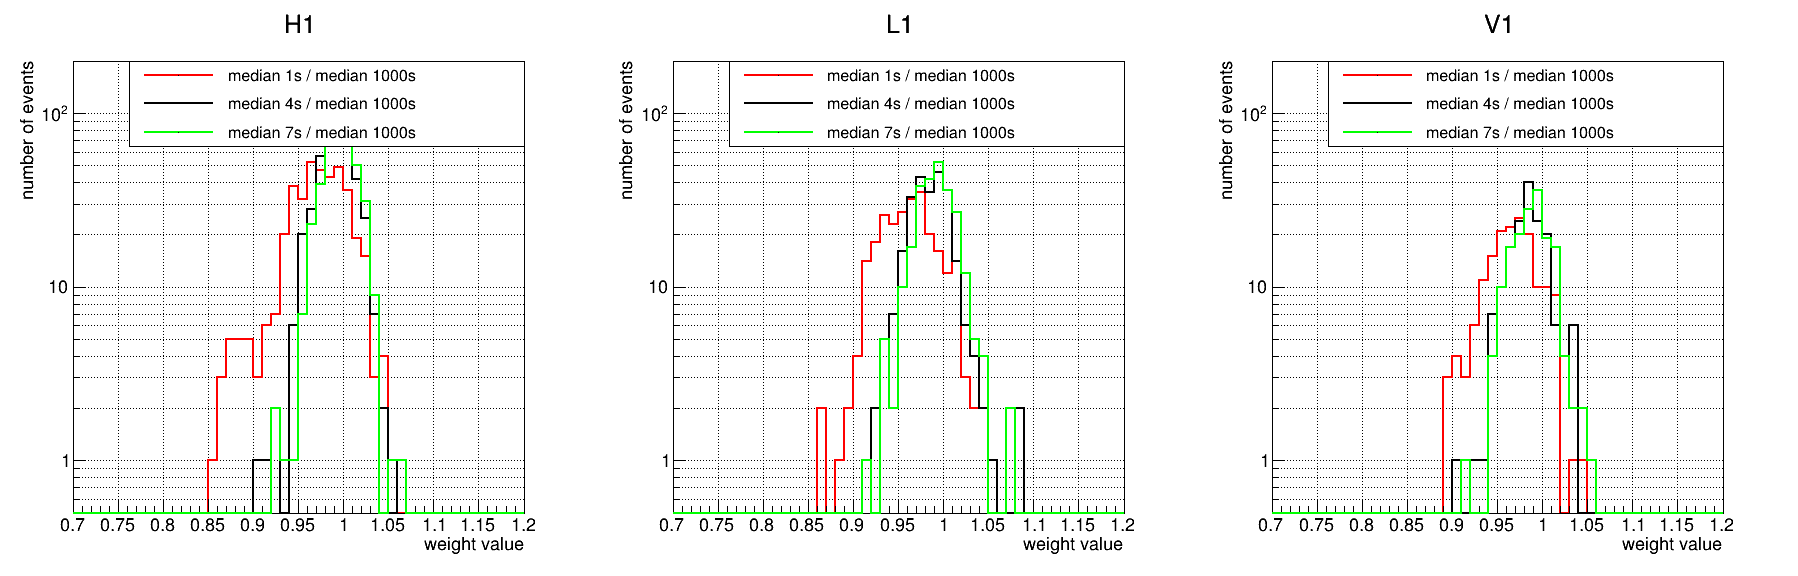
\includegraphics[width=\linewidth]{sectionBadTriggers/PSD/Reweight/cWeightDark.png}
%   \caption{Correction weights distribution for long EM dark singles}
%   \label{fig:weightDark}
% \end{figure}

% \begin{figure}[H]
%   \centering
%   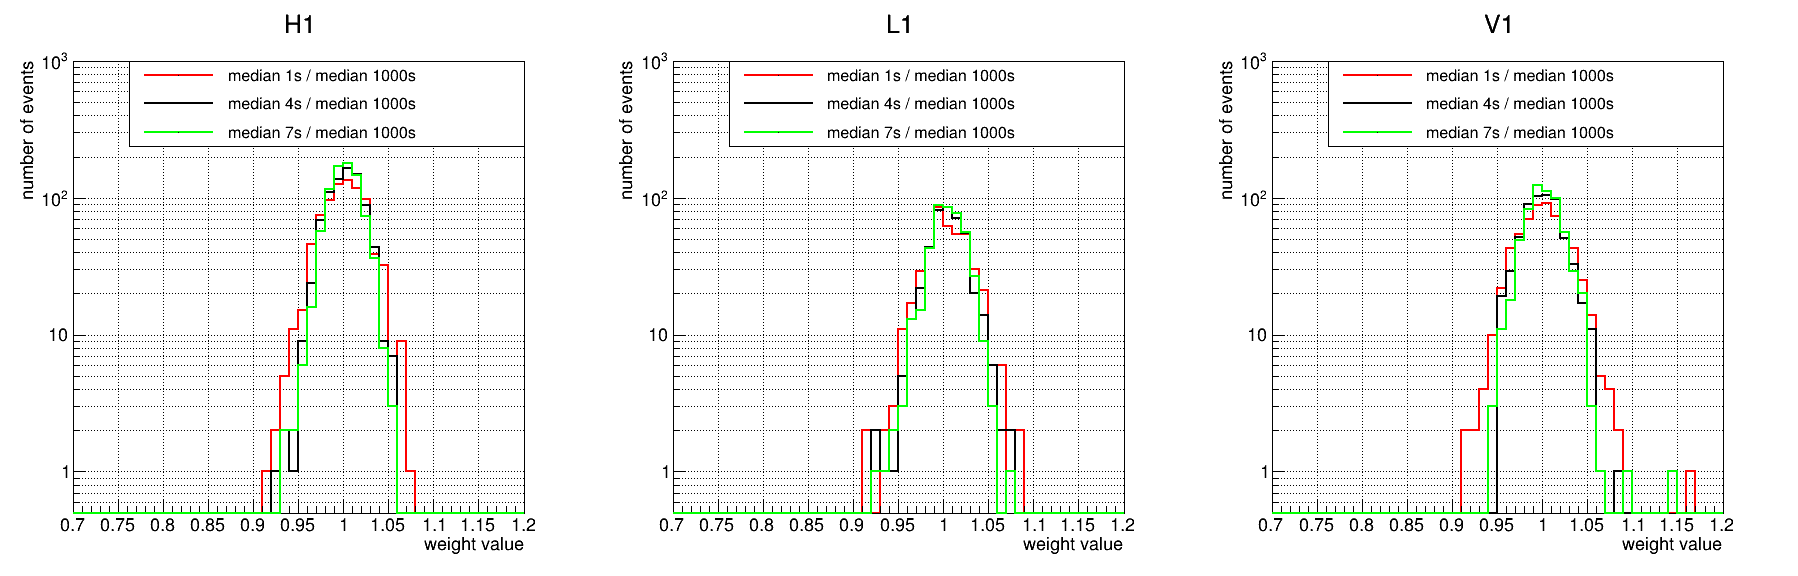
\includegraphics[width=\linewidth]{sectionBadTriggers/PSD/Reweight/cWeightRandomTimes.png}
%   \caption{Correction weights distribution for random times}
%   \label{fig:weightRandomTimes}
% \end{figure}





%%%%%%%%%%%%%%%%%%%%%%%%%%%%%%%%%%%%%%%%%%%%%%%%%%%%%%%%%%%%%%%%% 
%%%%%%%%%%%%%%%%%%%%%%%%%%%%%%%%%%%%%%%%%%%%%%%%%%%%%%%%%%%%%%%%% 
%%%%%%%%%%%%%%%%%%%%%%%%%%%%%%%%%%%%%%%%%%%%%%%%%%%%%%%%%%%%%%%%% 

%%%%%%% RANGE REAL DATA VS GAUSSIAN NOISE

\clearpage
\newpage
\subsection{Detector range: real data vs Gaussian noise}
\label{sec:range_real_vs_gaus}

We have seen that by studying the variations of the range for the gating, we were able to identify an issue that increases our background.
We wonder if there is more that can be learned.
We decide this time to have a look at the range itself (not the \medr{}).
 
It was shown that MBTA single detector triggers are quite far from the Gaussian noise level, although we were able to reduce this difference in chapter \ref{section:selection}.
We decide to investigate the differences in the range computed on real data compared to the range computed on Gaussian noise.
The goal is not to propose a solution to fix specific issues but rather to highlight possible discrepancies in the amplitude and time scale of the variations of the range which could be studied in the future.
 
We start by having a look at the BNS range, computed for a $1.4+1.4\msun$ system starting at a frequency of \SI{10}{Hz}.
The evolution of the range in time and frequency for real data and Gaussian noise are shown in figure \ref{fig:rangeReal_BNS_10} and \ref{fig:rangeGaus_BNS_10} respectively.
We show the range for several decimation factors because it allows to be more sensitive to low frequency fluctuations, especially in the time domain, since we expect differences to be at low frequencies.
The first thing we notice is the presence of many drops in the range computed on real data due to glitches and the absence of such drops in the range computed on Gaussian noise.
We also see that there are more fluctuations on large time scales in the range computed on real data, characterized by an excess in the (average) ASD for frequencies smaller than \SI{0.2}{Hz} when compared to the ASD of the range computed on Gaussian noise.
The ASD of the range computed on real data also decreases slightly from \SI{0.2}{Hz} to \SI{1}{Hz} while the ASD of the range computed on Gaussian noise is flatter.
The ASDs are however rather similar for higher frequencies with a drop around 4 Hz, corresponding to the time window (\SI{0.25}{s}) of the FFT used to compute the instantanious range (reminder: this time window is shifted by a step of \SI{1/32}{s} to compute a range at \SI{32}{Hz}).
 
Figures \ref{fig:rangeReal_BNS_10_1D} and \ref{fig:rangeGaus_BNS_10_1D} show the 1-Dimensional projection of the range computed on real data and Gaussian noise respectively.
The mean value of the range is roughly the same for real data and generated Gaussian noise but the standard deviation is larger in the case of real data up to a factor 2 when using a decimation factor of 256.
 
We also show in figures \ref{fig:rangeReal_BNS_50} and \ref{fig:rangeGaus_BNS_50} the real data range and gaussian noise range as a function of time and frequency with starting frequency of \SI{50}{Hz}.
Starting the computation of the range at \SI{50}{Hz} reduces the difference between the two ranges at low frequency.
 
We now wonder wether a range computed on a BBH system of $30+30\msun$ ($\nu_{\text{ISCO}} \sim \SI{73}{Hz}$) will exhibit the same effect.
Figures \ref{fig:rangeReal_BBH_10} and \ref{fig:rangeGaus_BBH_10} show the time and frequency dependency of the range computed on real data and gaussian noise respectively.
Here again the ASD of the range computed on real data is higher at low frequencies but the difference is smaller than for the BNS range.
Looking at the 1-D projections in figures \ref{fig:rangeReal_BBH_10_1D} and \ref{fig:rangeGaus_BBH_10_1D}, the two ranges have close mean values but different standard deviations with increasing difference as the decimation factor grows.
Similarly to the BNS range, we show figures \ref{fig:rangeReal_BBH_50} and \ref{fig:rangeGaus_BBH_50} for the computation of the range starting at \SI{50}{Hz}.
As for the BNS range, this makes the difference between the two ASDs at low frequencies barely noticeable.  
  
This did not lead to any changes for O4.
The goal is only to highlight some behaviours that may be of more interest in the future.


%%%%%%%%%%%%%%%%%%%%%%%%%%%%%%%%%%%%%%%%%%%%%%%%%%%%%% 
%%%%%%%%%%%%%%%%%%%%%%%%%%%%%%%%%%%%%%%%%%%%%%%%%%%%%% 

% FIGURES PART 3


% Real data & Gaus BNS 10Hz
\begin{figure}
  \centering
  \begin{minipage}{\linewidth}
    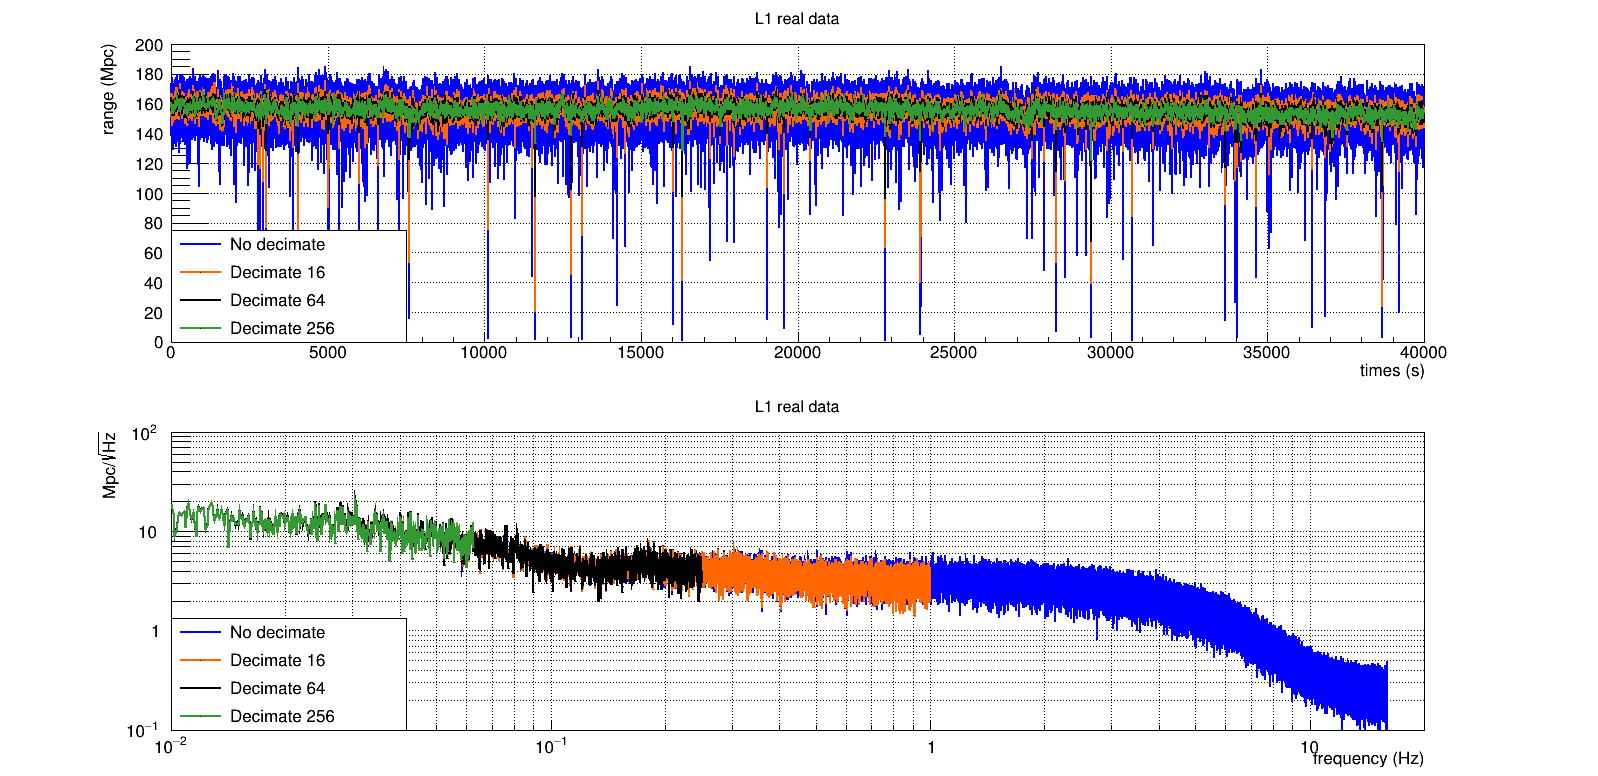
\includegraphics[width=\linewidth]{sectionBadTriggers/PSD/Range/range_PSD/cReal_L1_BNS.png}
    \caption{BNS range in the time and frequency domain, computed from 10Hz on real data}
    \label{fig:rangeReal_BNS_10}
  \end{minipage}
  \hfill
  \vspace{0.4cm}
  % 
  \begin{minipage}{\linewidth}
    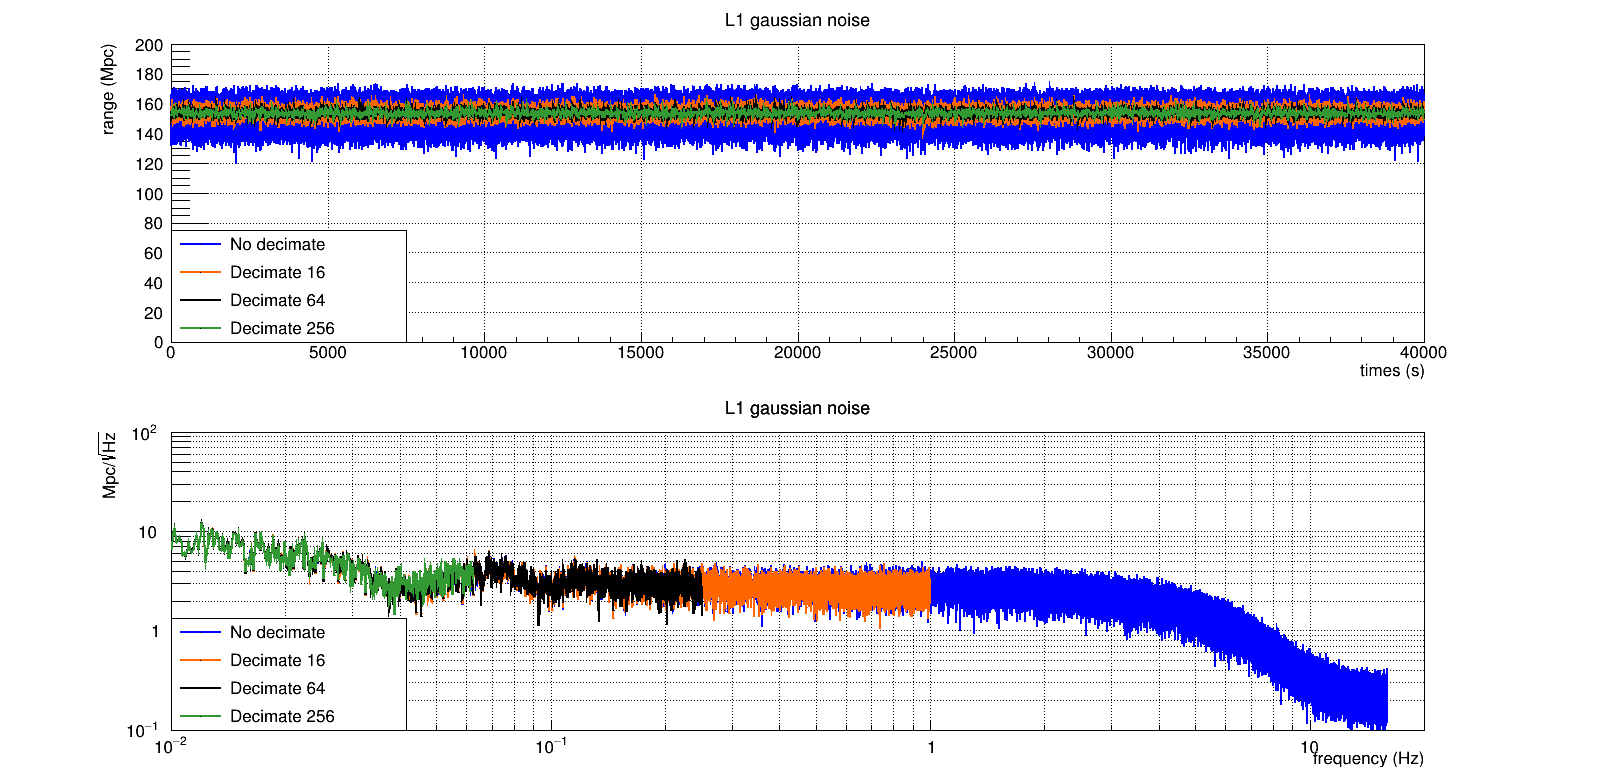
\includegraphics[width=\linewidth]{sectionBadTriggers/PSD/Range/range_PSD/cGaus_L1_BNS.png}
    \caption{BNS range in the time and frequency domain, computed from 10Hz on Gaussian noise}
    \label{fig:rangeGaus_BNS_10}
  \end{minipage}
\end{figure}


% Real data & Gaus BNS 10Hz histos
\begin{figure}
  \centering
  \begin{minipage}{\linewidth}
    \centering
    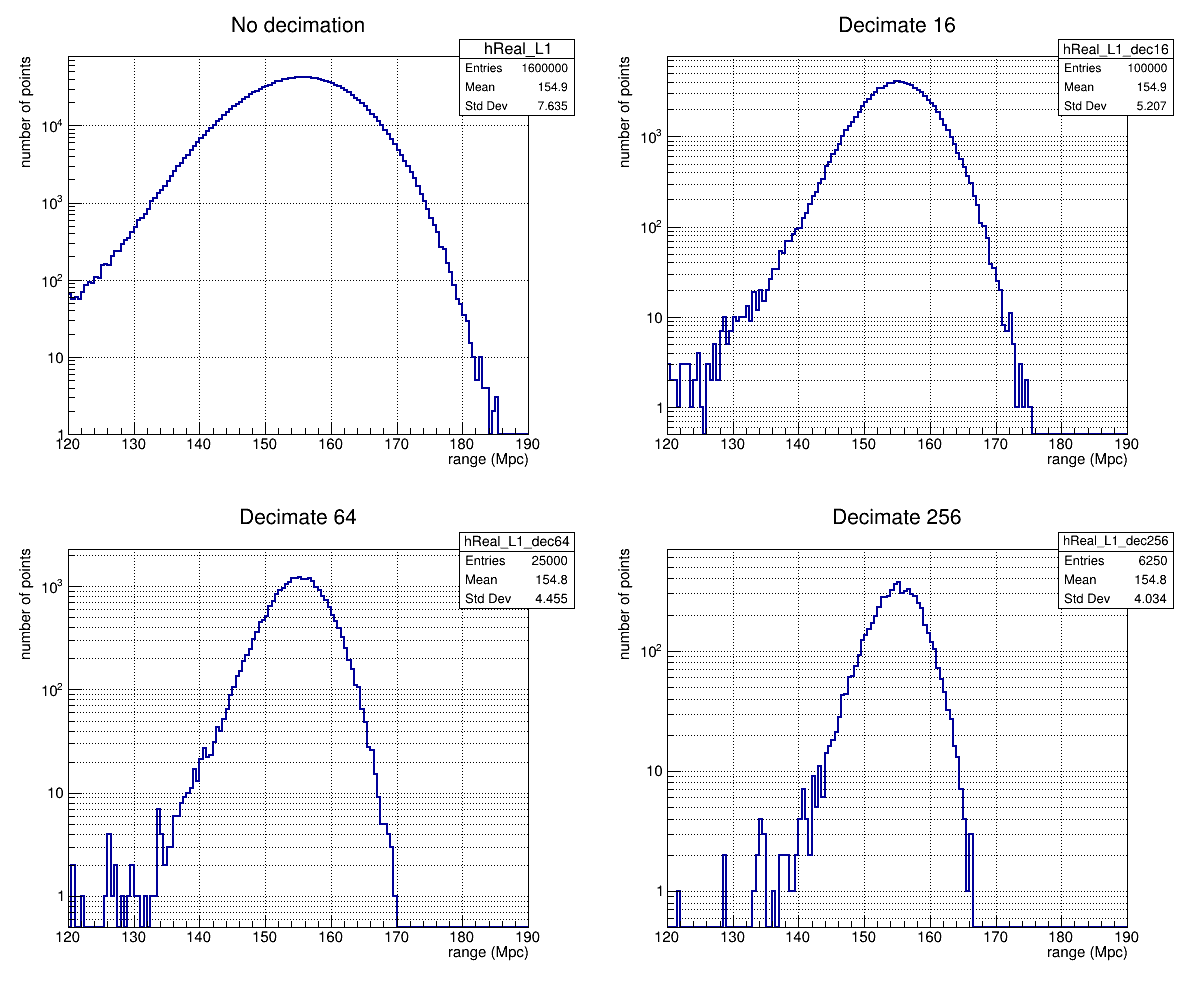
\includegraphics[width=0.7\linewidth]{sectionBadTriggers/PSD/Range/range_PSD/c1DReal_L1.png}
    \caption{1D projection of the BNS range in time domain computed from 10Hz on real data}
    \label{fig:rangeReal_BNS_10_1D}
  \end{minipage}
  \hfill
  \vspace{0.4cm}
  %
  \begin{minipage}{\linewidth}
    \centering
    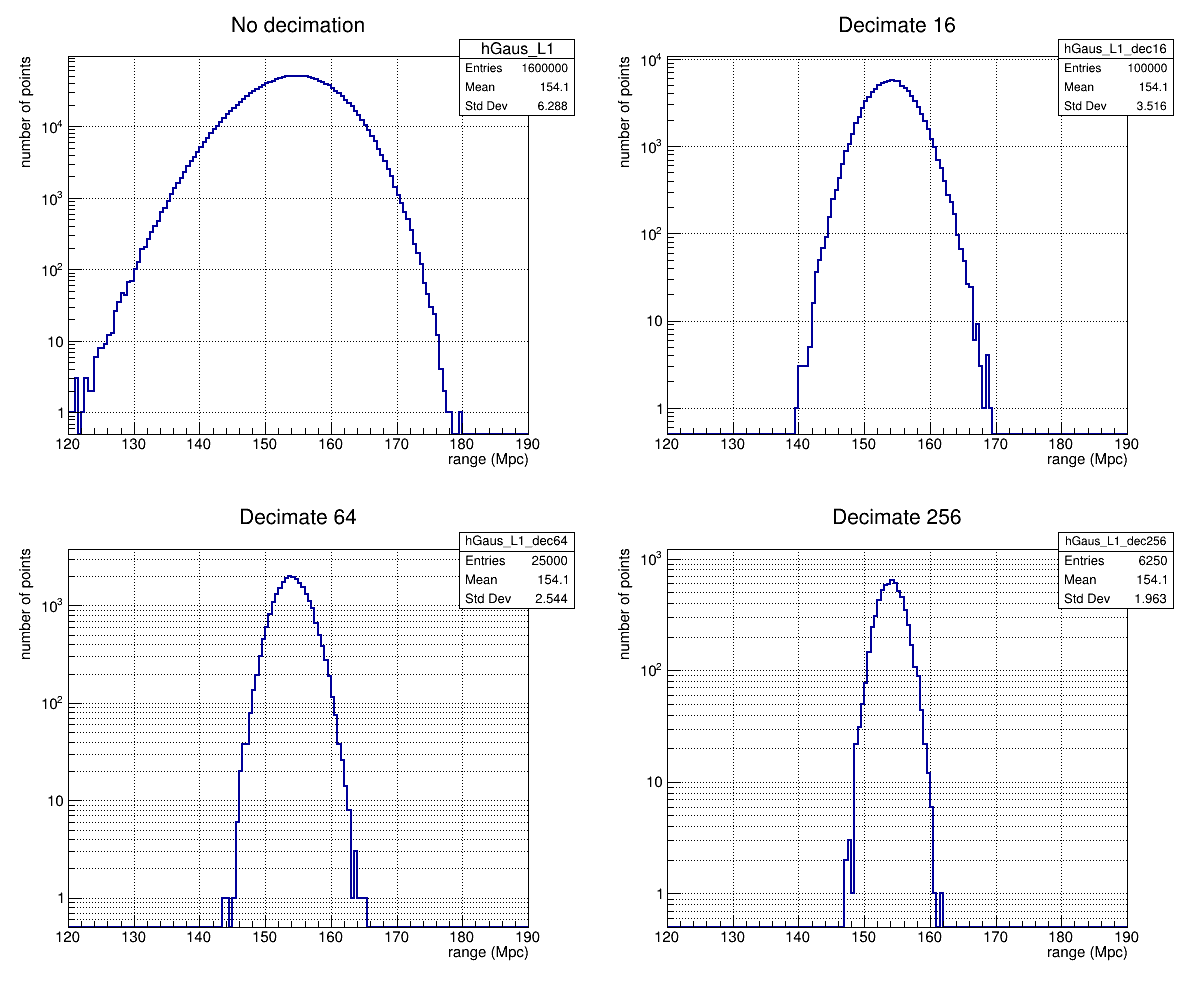
\includegraphics[width=0.7\linewidth]{sectionBadTriggers/PSD/Range/range_PSD/c1DGaus_L1.png}
    \caption{1D projection of the BNS range in time domain computed from 10Hz on Gaussian noise}
    \label{fig:rangeGaus_BNS_10_1D}
  \end{minipage}
\end{figure}

%
% Real data & Gaus BNS 20Hz
% \begin{figure}
%   \centering
%   \begin{minipage}{\linewidth}
%     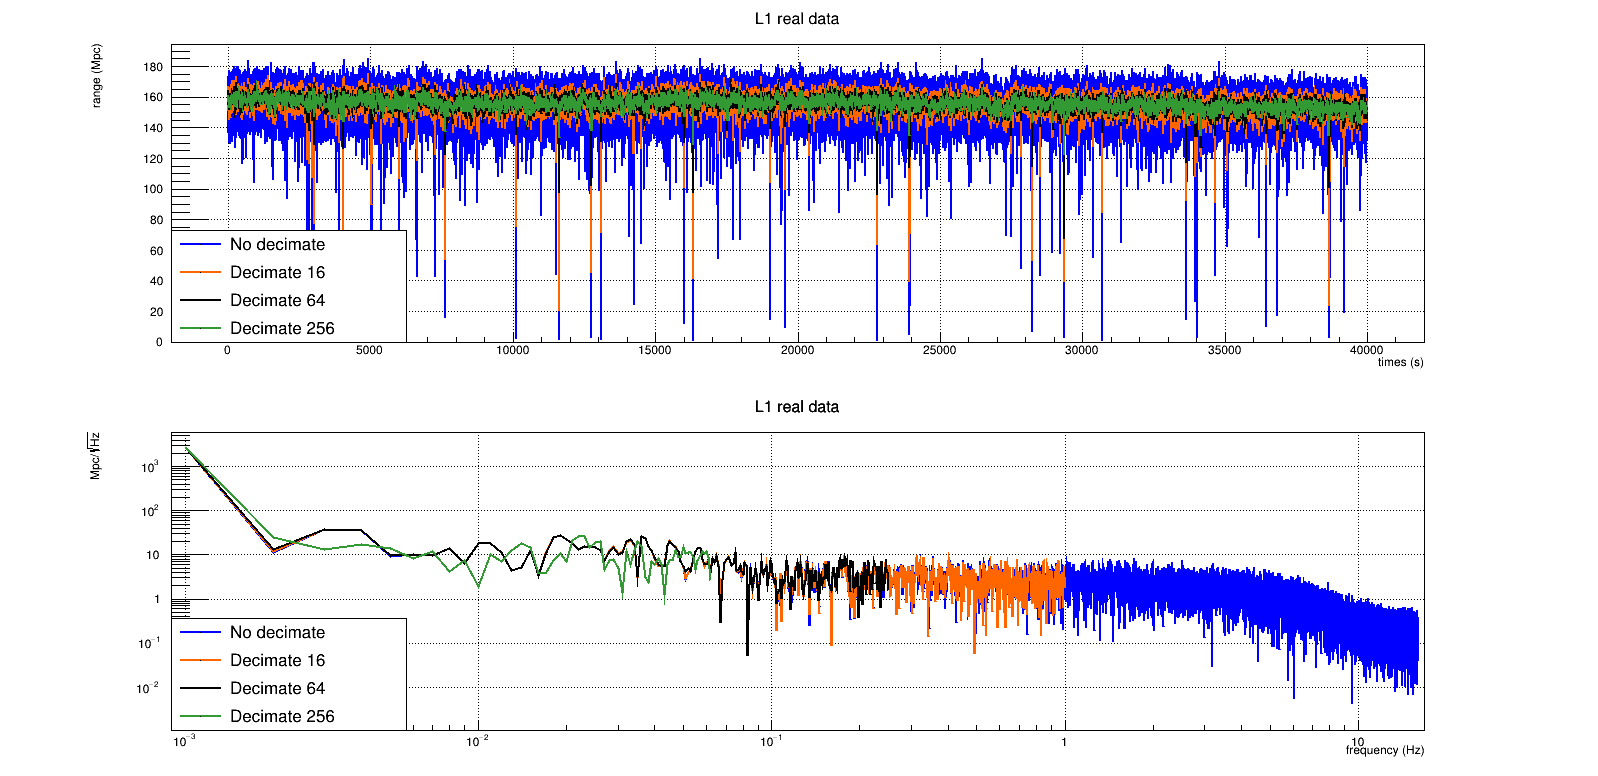
\includegraphics[width=\linewidth]{sectionBadTriggers/PSD/Range/range_PSD/cReal_L1_20Hz.png}
%     \caption{BNS range in the time and frequency domain, computed from 20Hz on real data}
%     \label{fig:rangeReal_BNS_20}
%   \end{minipage}
%   \hfill
%   \vspace{0.4cm}
%   % 
%   \begin{minipage}{\linewidth}
%     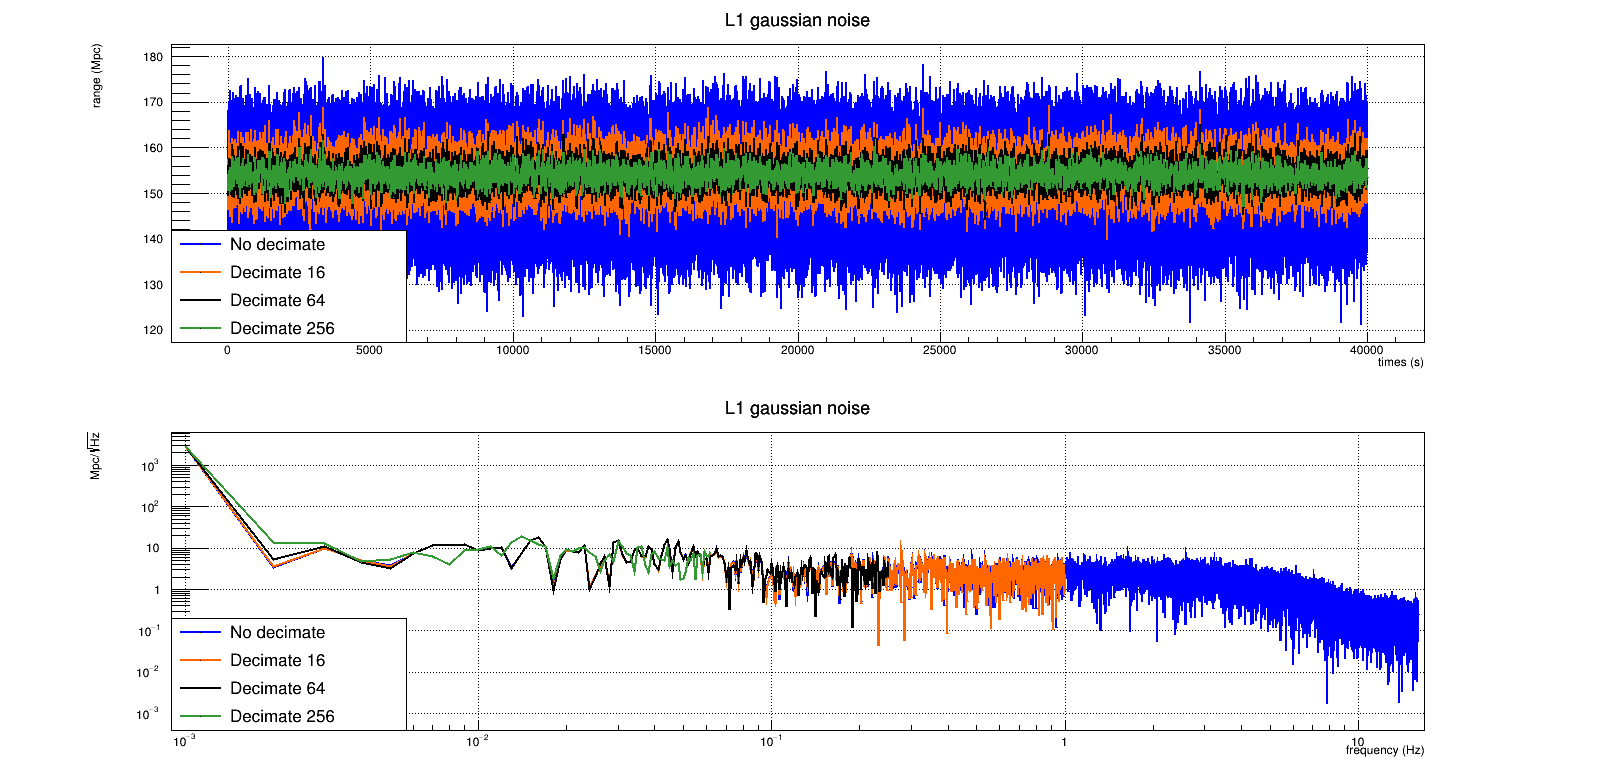
\includegraphics[width=\linewidth]{sectionBadTriggers/PSD/Range/range_PSD/cGaus_L1_20Hz.png}
%     \caption{BNS range in the time and frequency domain, computed from 20Hz on Gaussian noise}
%     \label{fig:rangeGaus_BNS_20}
%   \end{minipage}
% \end{figure}

% Real data & Gaus BNS 50Hz
\begin{figure}
  \centering
  \begin{minipage}{\linewidth}
    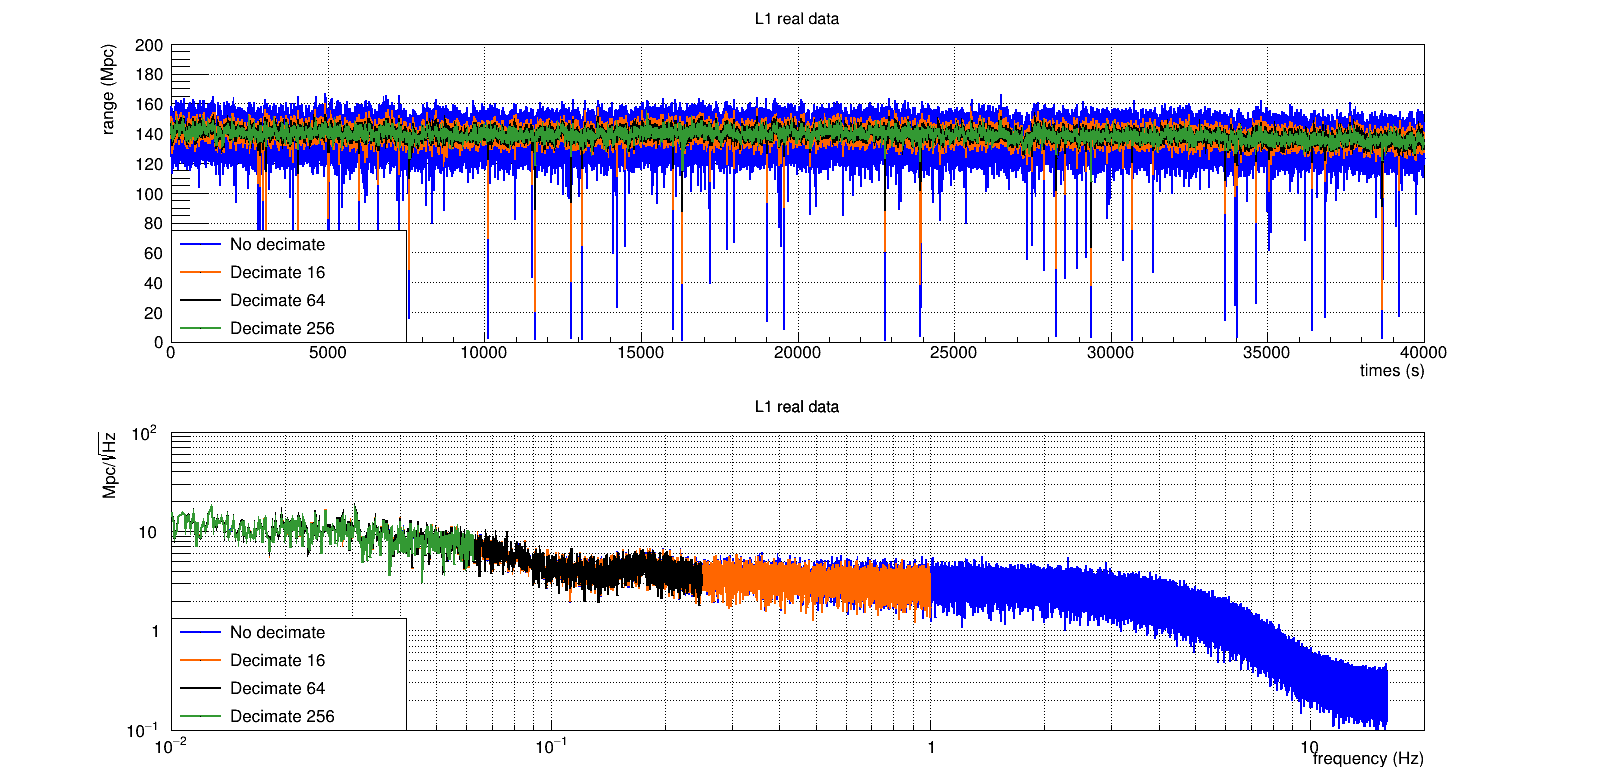
\includegraphics[width=\linewidth]{sectionBadTriggers/PSD/Range/range_PSD/cReal_L1_50Hz_BNS.png}
    \caption{BNS range in the time and frequency domain, computed from 50Hz on real data}
    \label{fig:rangeReal_BNS_50}
  \end{minipage}
  \hfill
  \vspace{0.4cm}
  % 
  \begin{minipage}{\linewidth}
    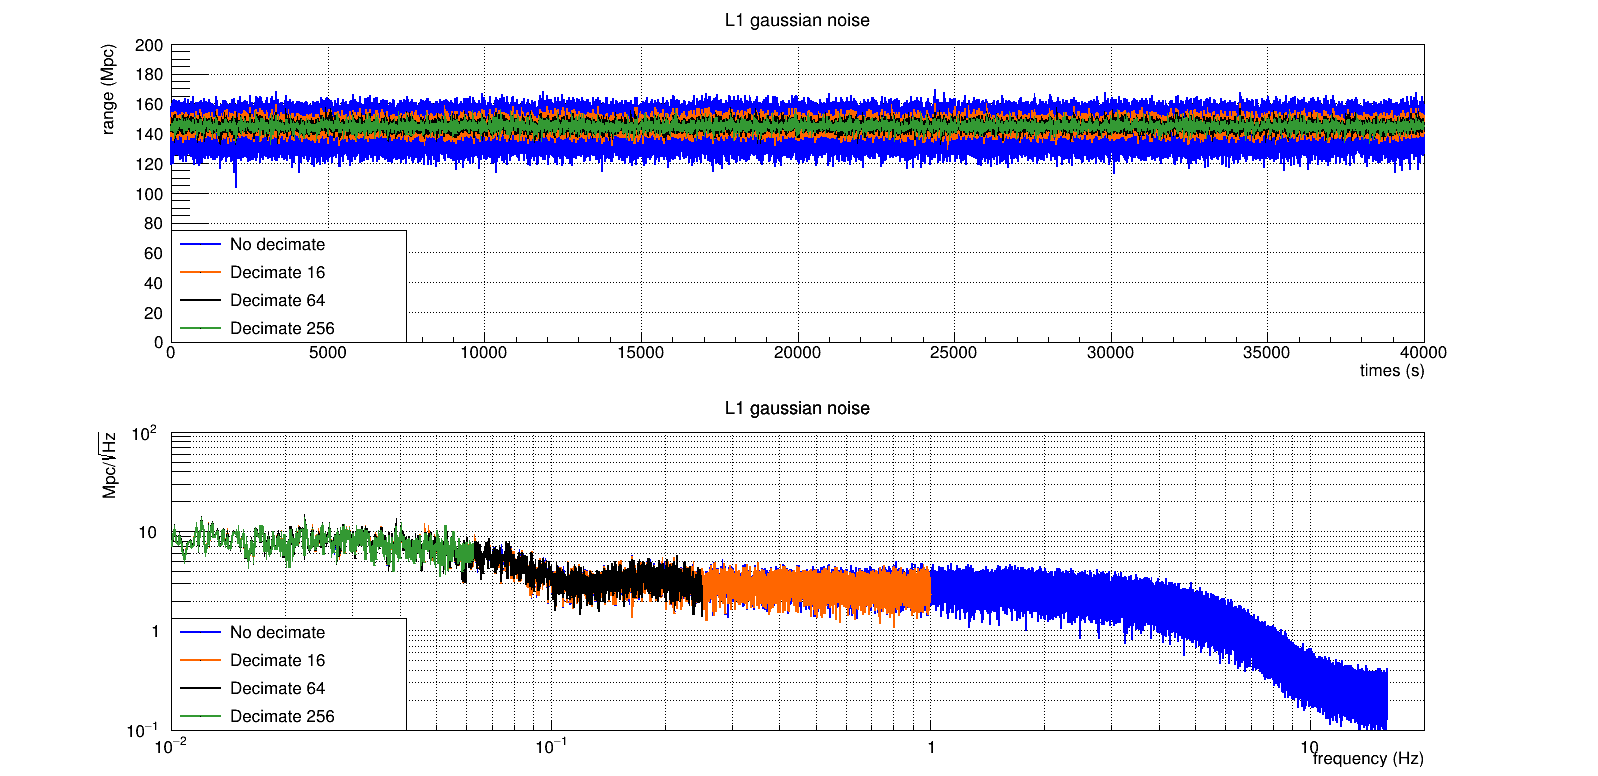
\includegraphics[width=\linewidth]{sectionBadTriggers/PSD/Range/range_PSD/cGaus_L1_50Hz_BNS.png}
    \caption{BNS range in the time and frequency domain, computed from 50Hz on Gaussian noise}
    \label{fig:rangeGaus_BNS_50}
  \end{minipage}
\end{figure}








% Real data & Gaus BBH 10Hz
\begin{figure}
  \centering
  \begin{minipage}{\linewidth}
    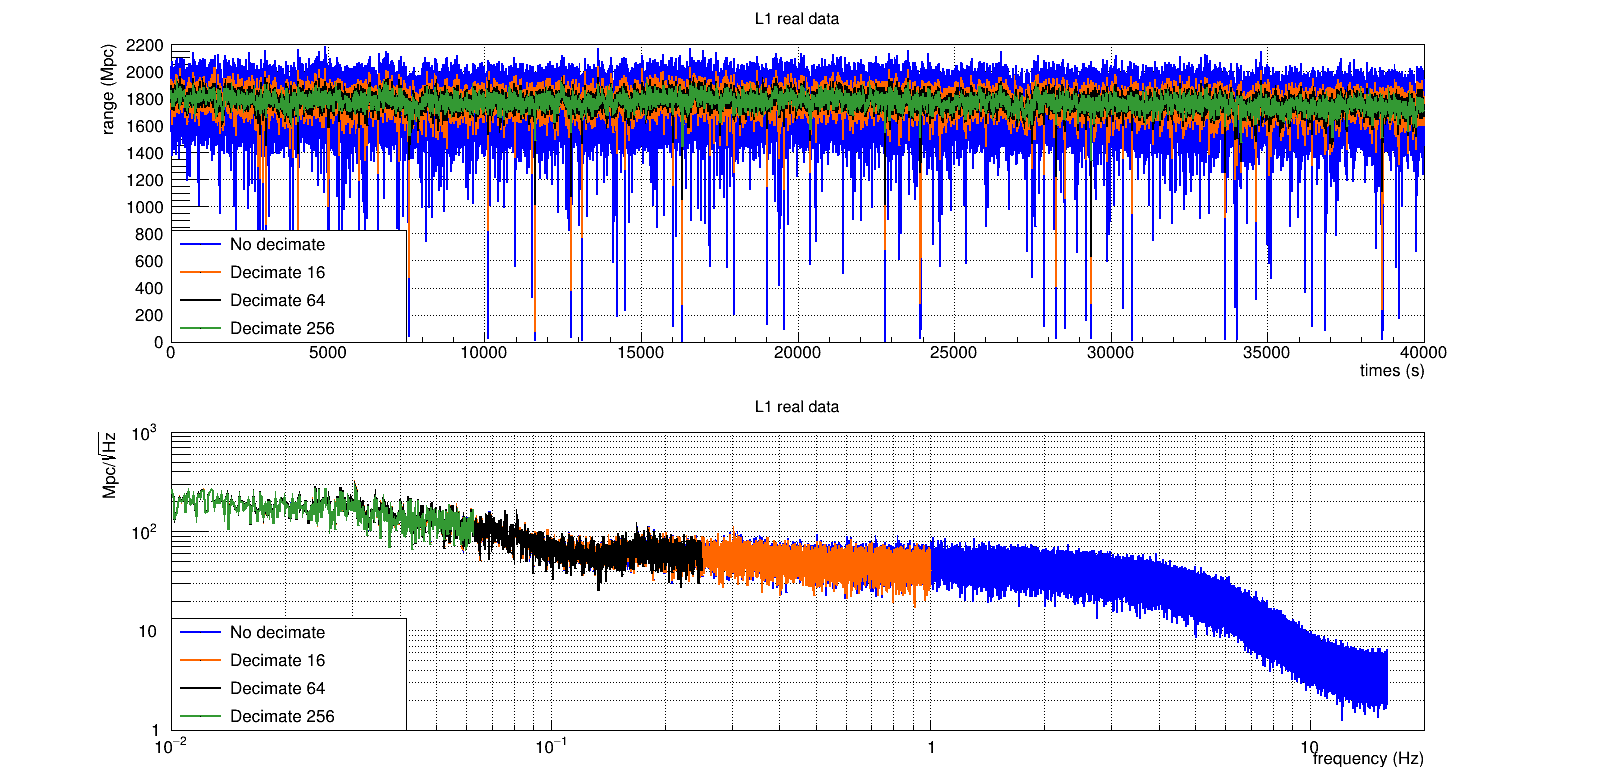
\includegraphics[width=\linewidth]{sectionBadTriggers/PSD/Range/range_PSD/cReal_L1_BBH.png}
    \caption{BBH range in the time and frequency domain, computed from 10Hz on real data}
    \label{fig:rangeReal_BBH_10}
  \end{minipage}
  \hfill
  \vspace{0.4cm}
  % 
  \begin{minipage}{\linewidth}
    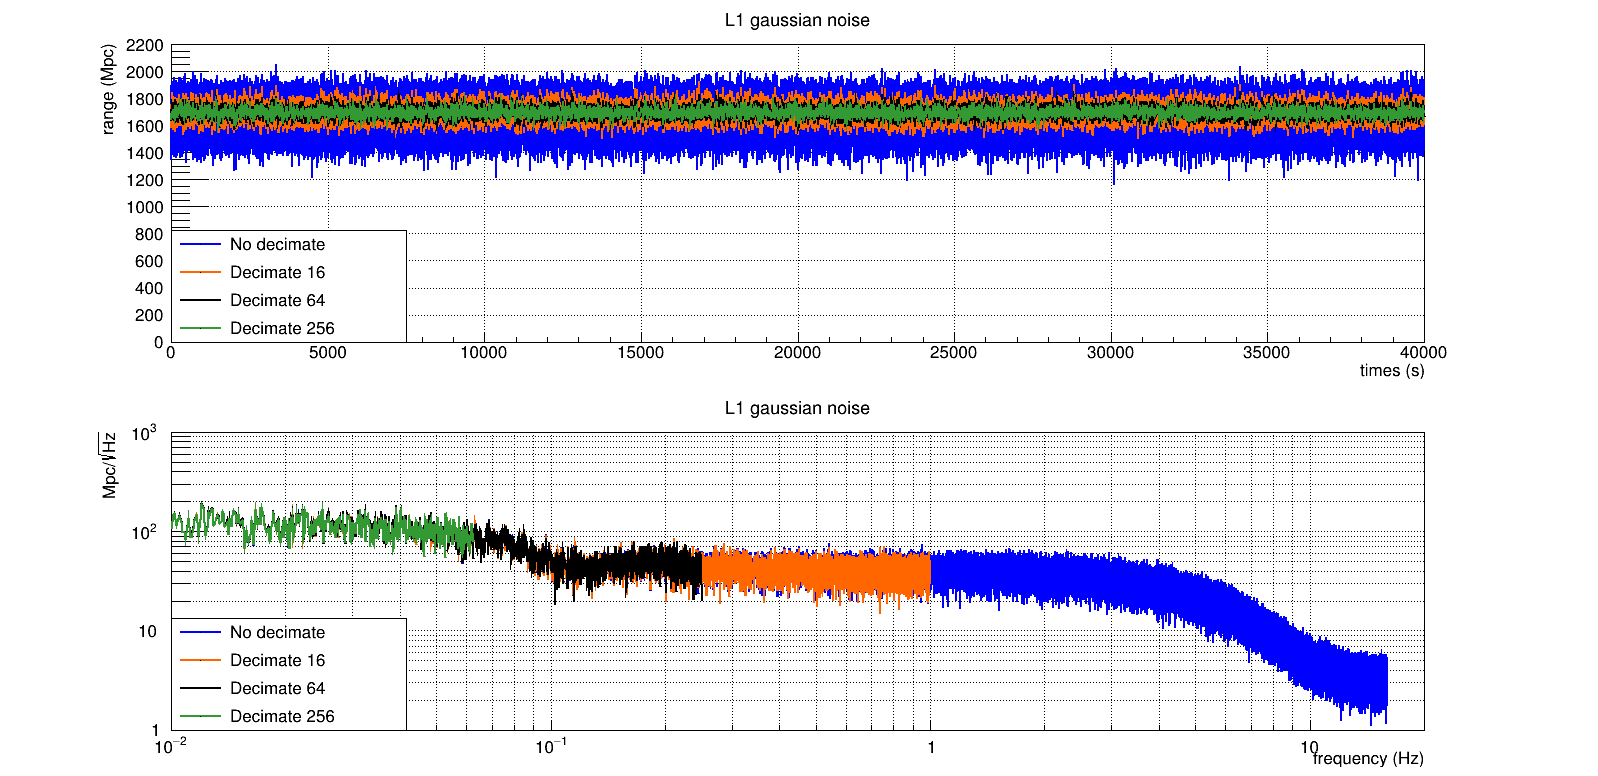
\includegraphics[width=\linewidth]{sectionBadTriggers/PSD/Range/range_PSD/cGaus_L1_BBH.png}
    \caption{BBH range in the time and frequency domain, computed from 10Hz on Gaussian noise}
    \label{fig:rangeGaus_BBH_10}
  \end{minipage}
\end{figure}


% Real data & Gaus BBH 10Hz histos
\begin{figure}
  \centering
  \begin{minipage}{\linewidth}
    \centering
    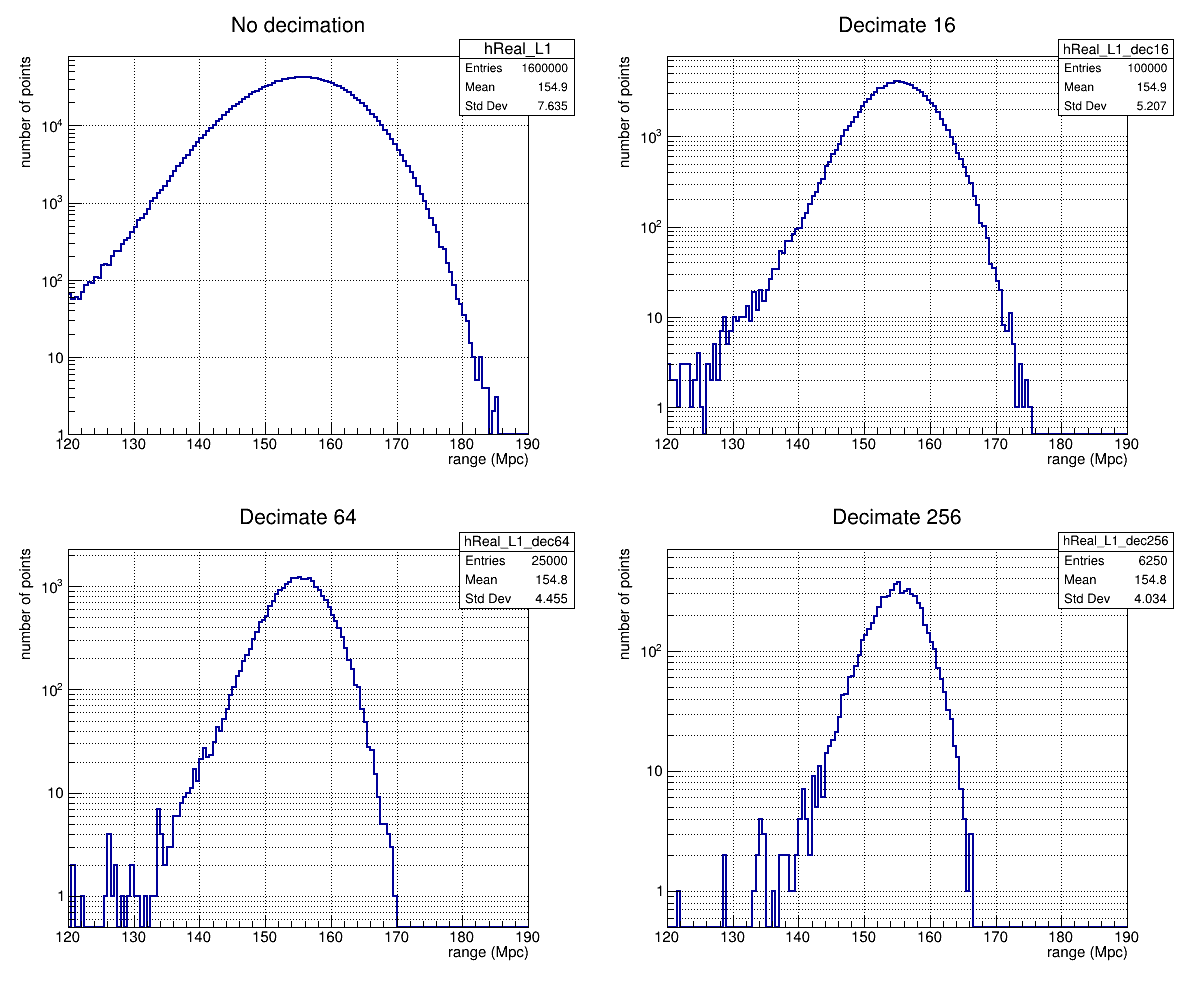
\includegraphics[width=0.7\linewidth]{sectionBadTriggers/PSD/Range/range_PSD/c1DReal_L1.png}
    \caption{1D projection of the BBH range in time domain computed from 10Hz on real data}
    \label{fig:rangeReal_BBH_10_1D}
  \end{minipage}
  \hfill
  \vspace{0.4cm}
  %
  \begin{minipage}{\linewidth}
    \centering
    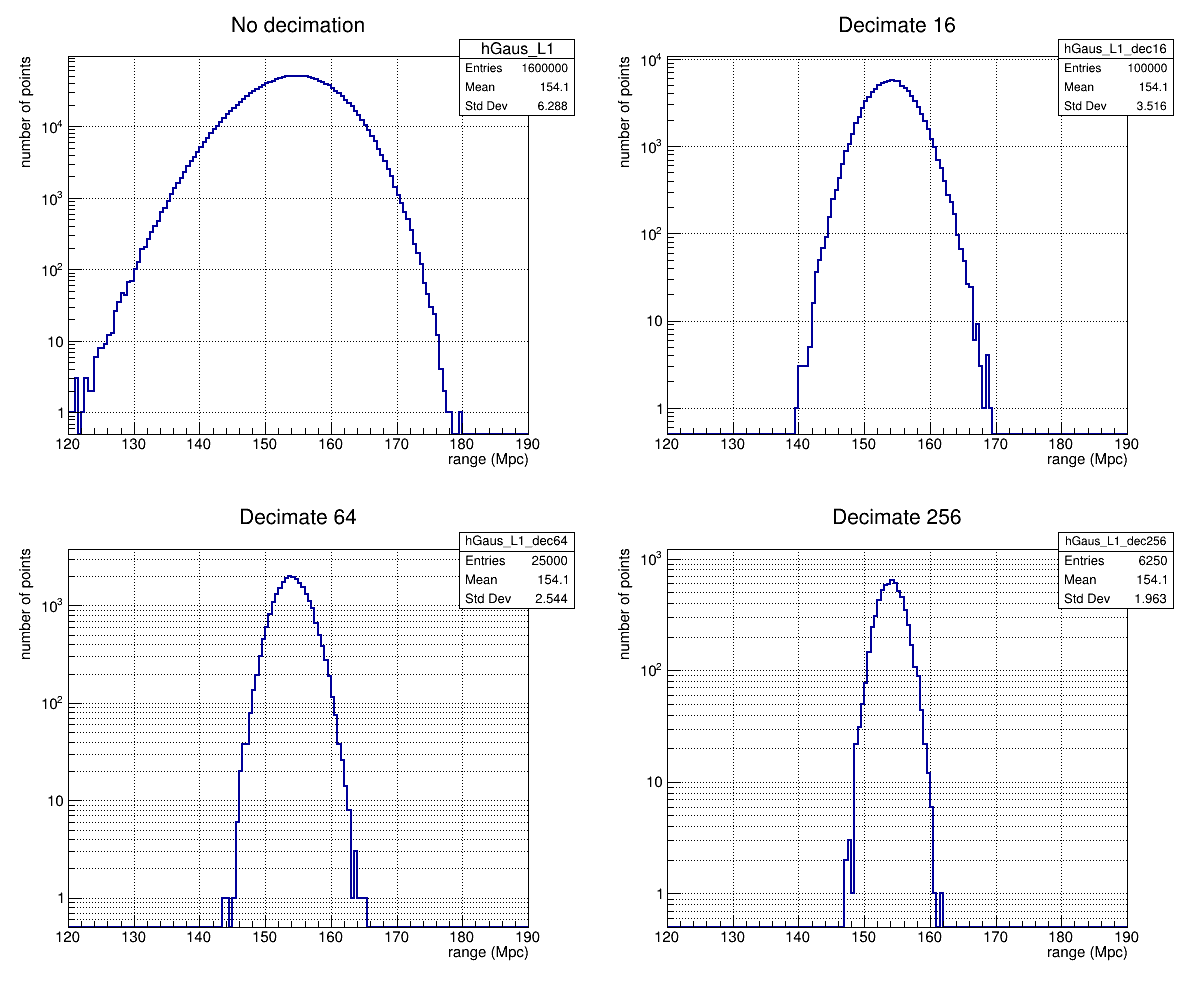
\includegraphics[width=0.7\linewidth]{sectionBadTriggers/PSD/Range/range_PSD/c1DGaus_L1.png}
    \caption{1D projection of the BBH range in time domain computed from 10Hz on Gaussian noise}
    \label{fig:rangeGaus_BBH_10_1D}
  \end{minipage}
\end{figure}

%
% Real data & Gaus BBH 20Hz
% \begin{figure}
%   \centering
%   \begin{minipage}{\linewidth}
%     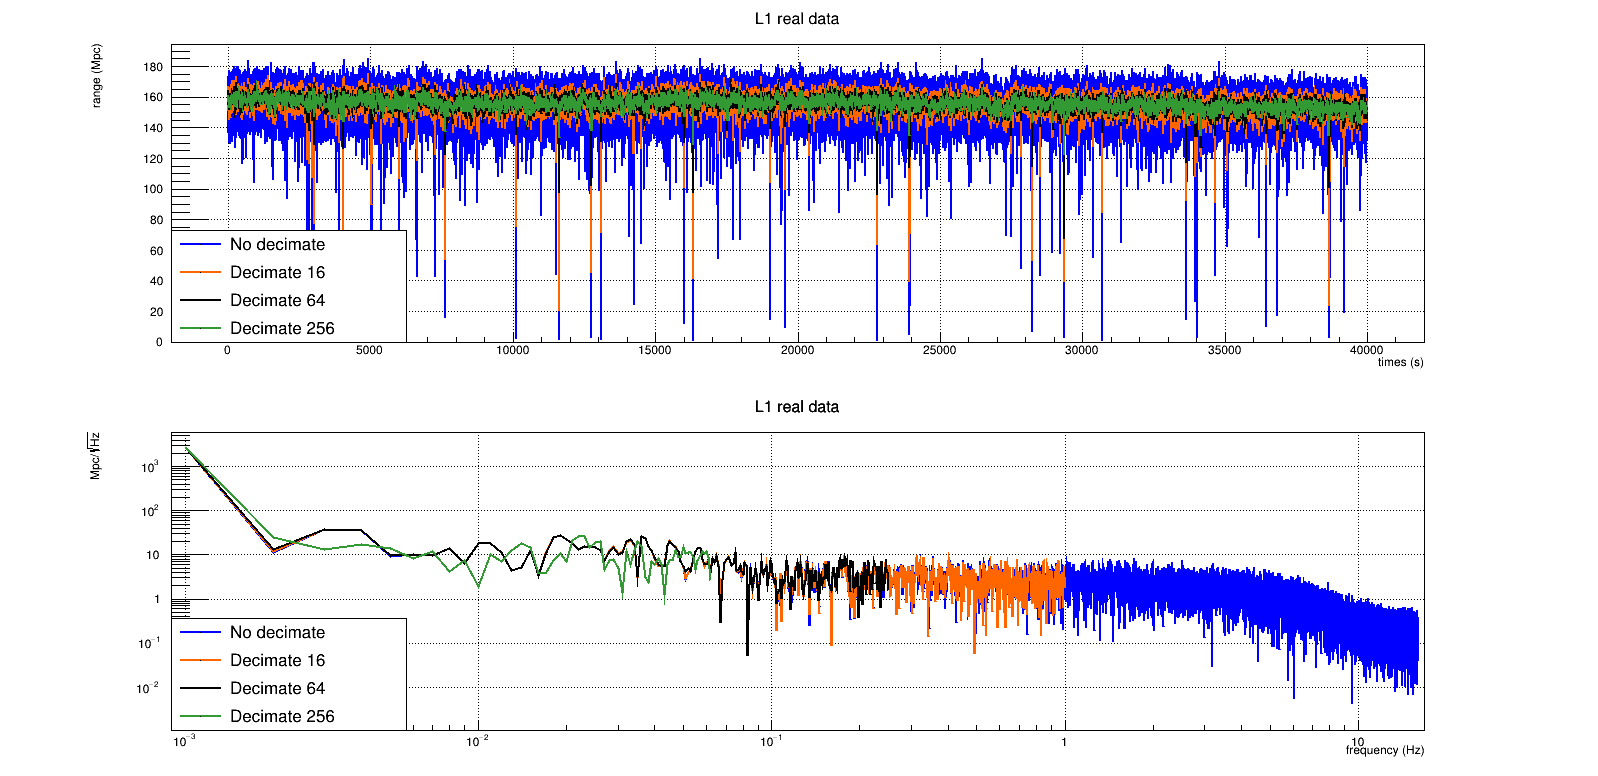
\includegraphics[width=\linewidth]{sectionBadTriggers/PSD/Range/range_PSD/cReal_L1_20Hz.png}
%     \caption{BBH range in the time and frequency domain, computed from 20Hz on real data}
%     \label{fig:rangeReal_BBH_20}
%   \end{minipage}
%   \hfill
%   \vspace{0.4cm}
%   % 
%   \begin{minipage}{\linewidth}
%     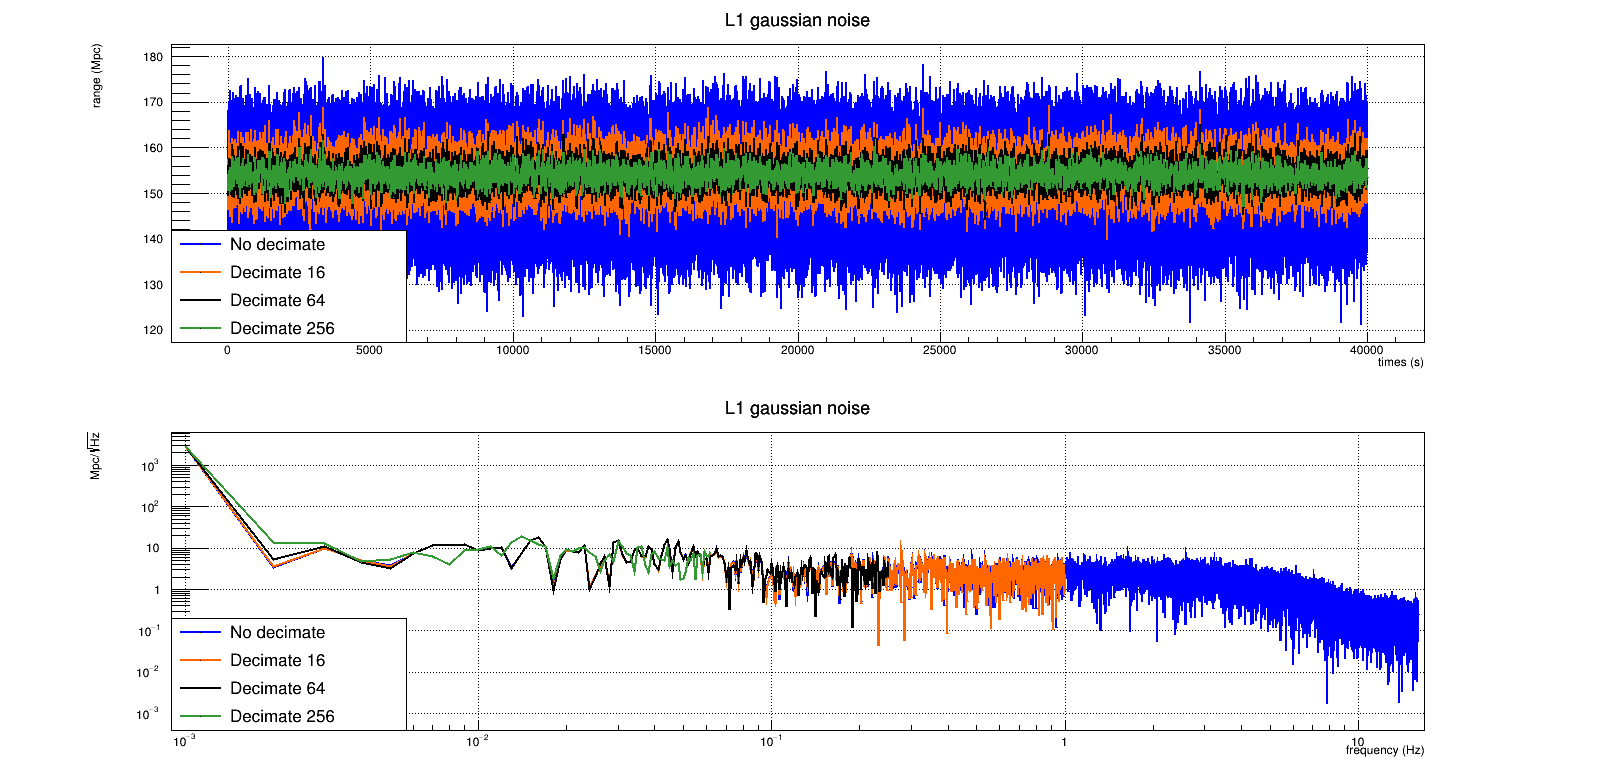
\includegraphics[width=\linewidth]{sectionBadTriggers/PSD/Range/range_PSD/cGaus_L1_20Hz.png}
%     \caption{BBH range in the time and frequency domain, computed from 20Hz on Gaussian noise}
%     \label{fig:rangeGaus_BBH_20}
%   \end{minipage}
% \end{figure}

% Real data & Gaus BBH 50Hz
\begin{figure}
  \centering
  \begin{minipage}{\linewidth}
    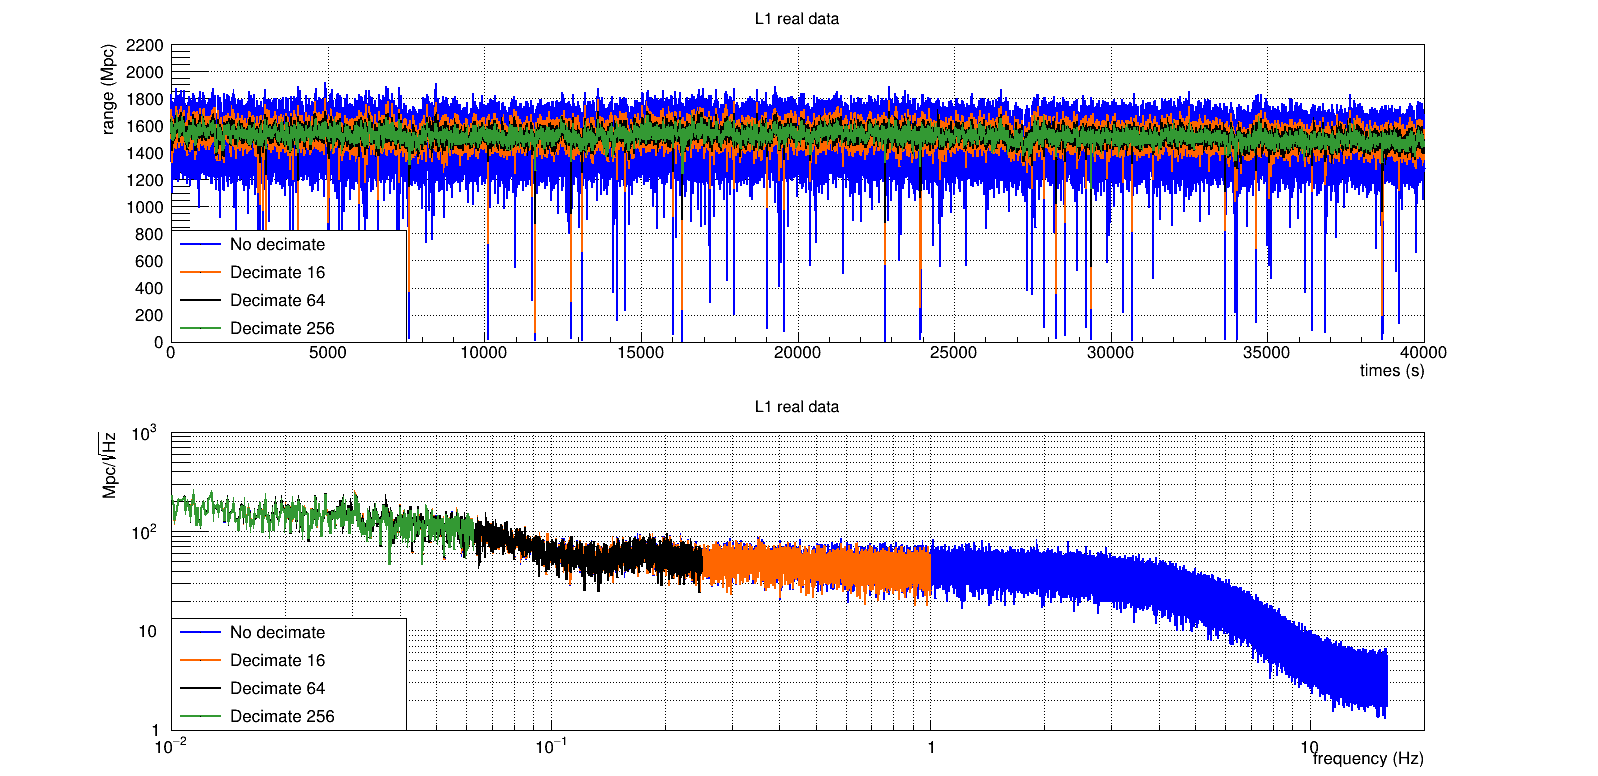
\includegraphics[width=\linewidth]{sectionBadTriggers/PSD/Range/range_PSD/cReal_L1_50Hz_BBH.png}
    \caption{BBH range in the time and frequency domain, computed from 50Hz on real data}
    \label{fig:rangeReal_BBH_50}
  \end{minipage}
  \hfill
  \vspace{0.4cm}
  % 
  \begin{minipage}{\linewidth}
    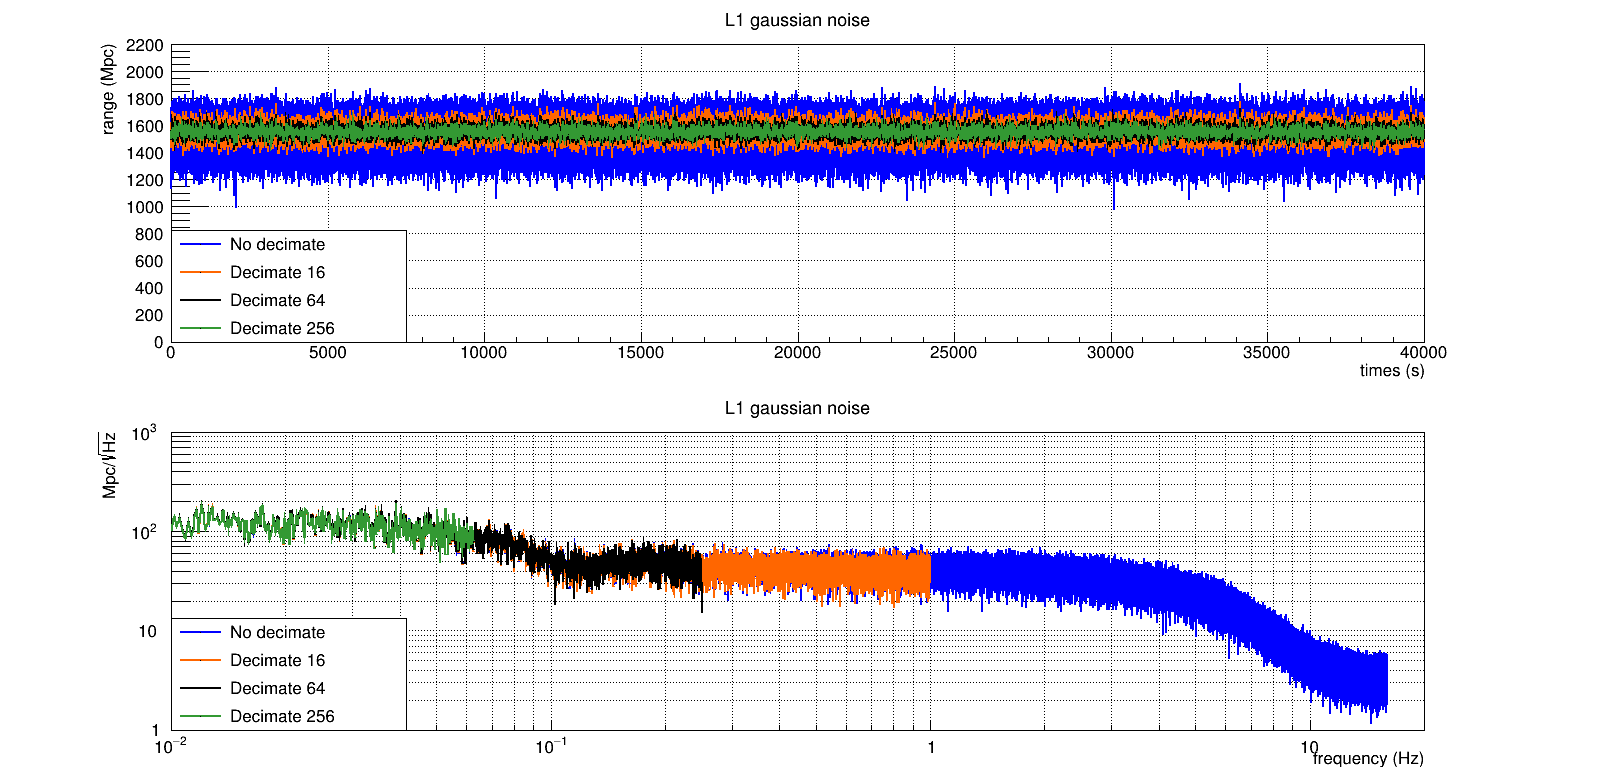
\includegraphics[width=\linewidth]{sectionBadTriggers/PSD/Range/range_PSD/cGaus_L1_50Hz_BBH.png}
    \caption{BBH range in the time and frequency domain, computed from 50Hz on Gaussian noise}
    \label{fig:rangeGaus_BBH_50}
  \end{minipage}
\end{figure}



%%%%%%%%%%%%%%%%%%%%%%%%%%%%%%%%%%%%%%%%%%%%%%%%%%%%%%%%%%%%%%%%%%%%%%%%%%%%%%%%%%%%%%%%%%%%%%%%%%%%%%%%%%%%%%%%%%%%%%%%%%%%%%%%%%%%%%%%%%%%%%%%%%%%%%%%%%%% ù
%%%%%%%%%%%%%%%%%%%%%%%%%%%%%%%%%%%%%%%%%%%%%%%%%%%%%%%%%%%%%%%%%%%%%%%%%%%%%%%%%%%%%%%%%%%%%%%%%%%%%%%%%%%%%%%%%%%%%%%%%%%%%%%%%%%%%%%%%%%%%%%%%%%%%%%%%%%%%%

% % Real data BBH
% \begin{figure}[H]
%   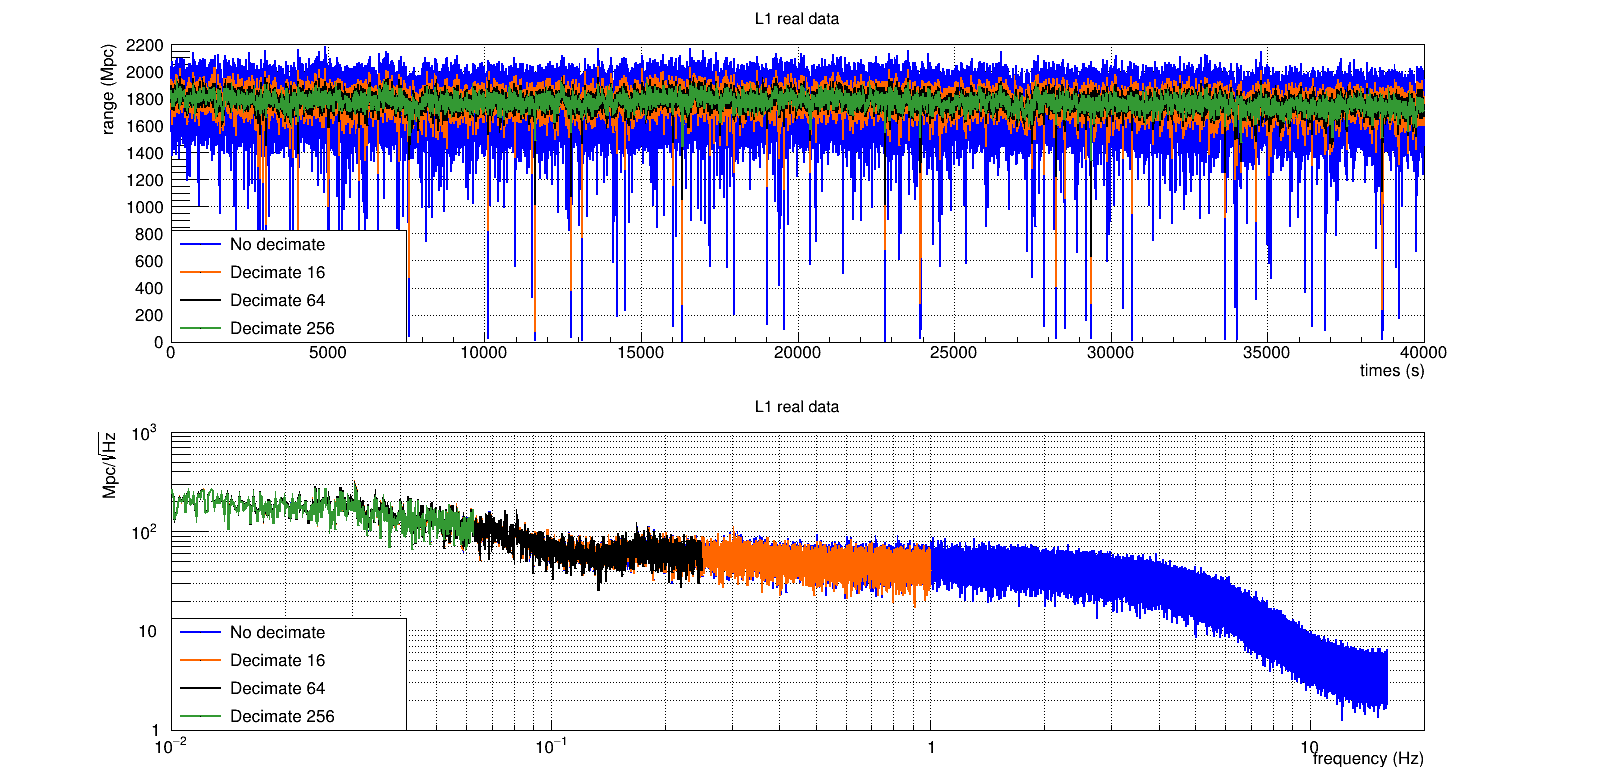
\includegraphics[width=\linewidth]{sectionBadTriggers/PSD/Range/range_PSD/cReal_L1_BBH.png}
%   \captionof{figure}{BBH range in the time and frequency domain, computed from 10Hz on real data}
%   \label{fig:rangeReal_BBH_10}
% \end{figure}
% % 
% \begin{figure}[H]
%   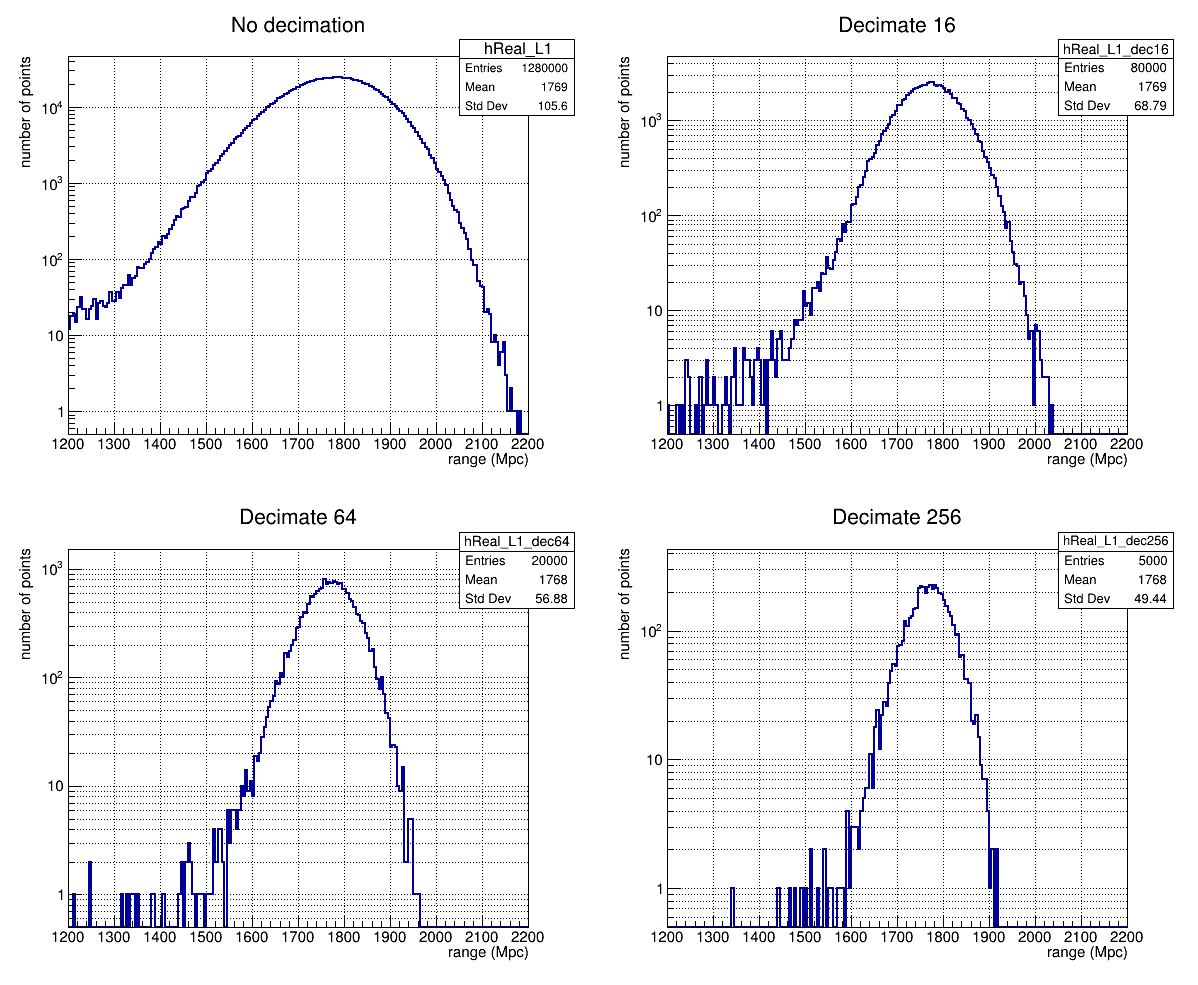
\includegraphics[width=\linewidth]{sectionBadTriggers/PSD/Range/range_PSD/c1DReal_L1_BBH.png}
%   \captionof{figure}{1D projection of the BBH range in time domain computed from 10Hz on real data}
%   \label{fig:rangeReal_BBH_10_1D}
% \end{figure}
% % 
% \begin{figure}[H]
%   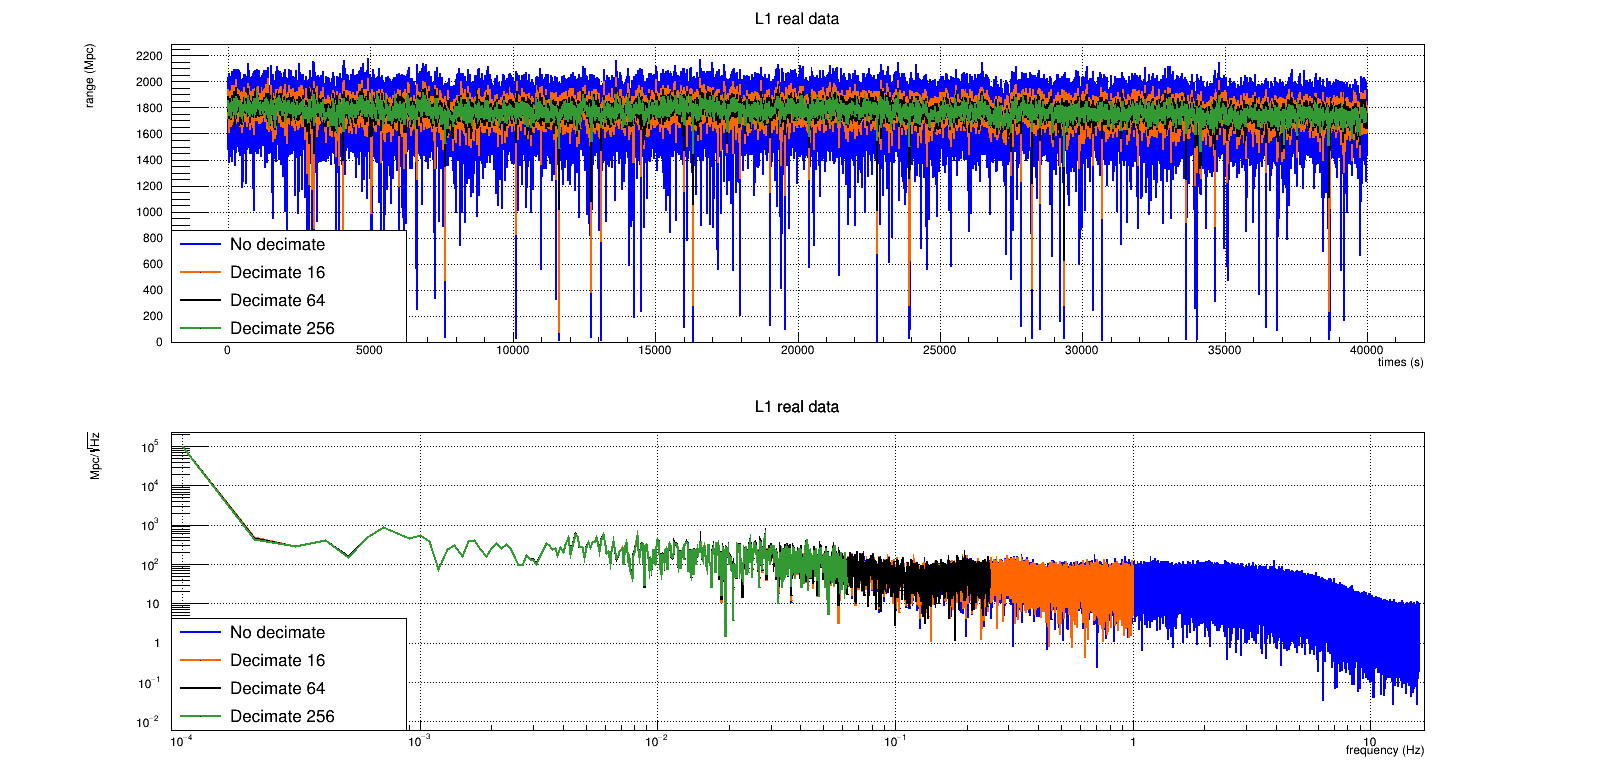
\includegraphics[width=\linewidth]{sectionBadTriggers/PSD/Range/range_PSD/cReal_L1_BBH_20Hz.png}
%   \captionof{figure}{BBH range in the time and frequency domain, computed from 20Hz on real data}
%   \label{fig:rangeReal_BBH_20}
% \end{figure}
% % 
% \begin{figure}[H]
%   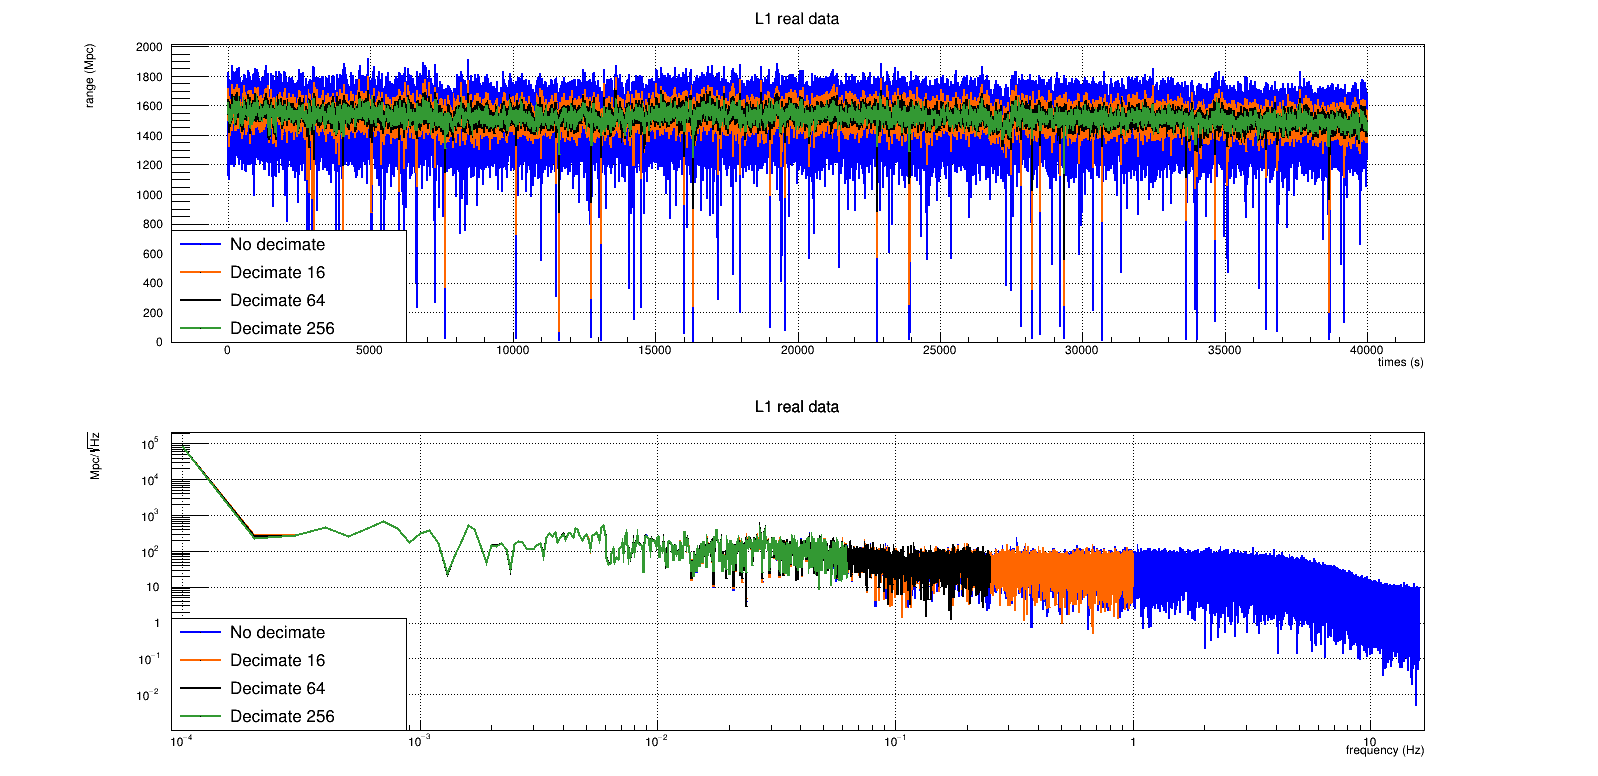
\includegraphics[width=\linewidth]{sectionBadTriggers/PSD/Range/range_PSD/cReal_L1_BBH_50Hz.png}
%   \captionof{figure}{BBH range in the time and frequency domain, computed from 50Hz on real data}
%   \label{fig:rangeReal_BBH_50}
% \end{figure}








% % Gaussian noise BBH
% \begin{figure}[H]
%   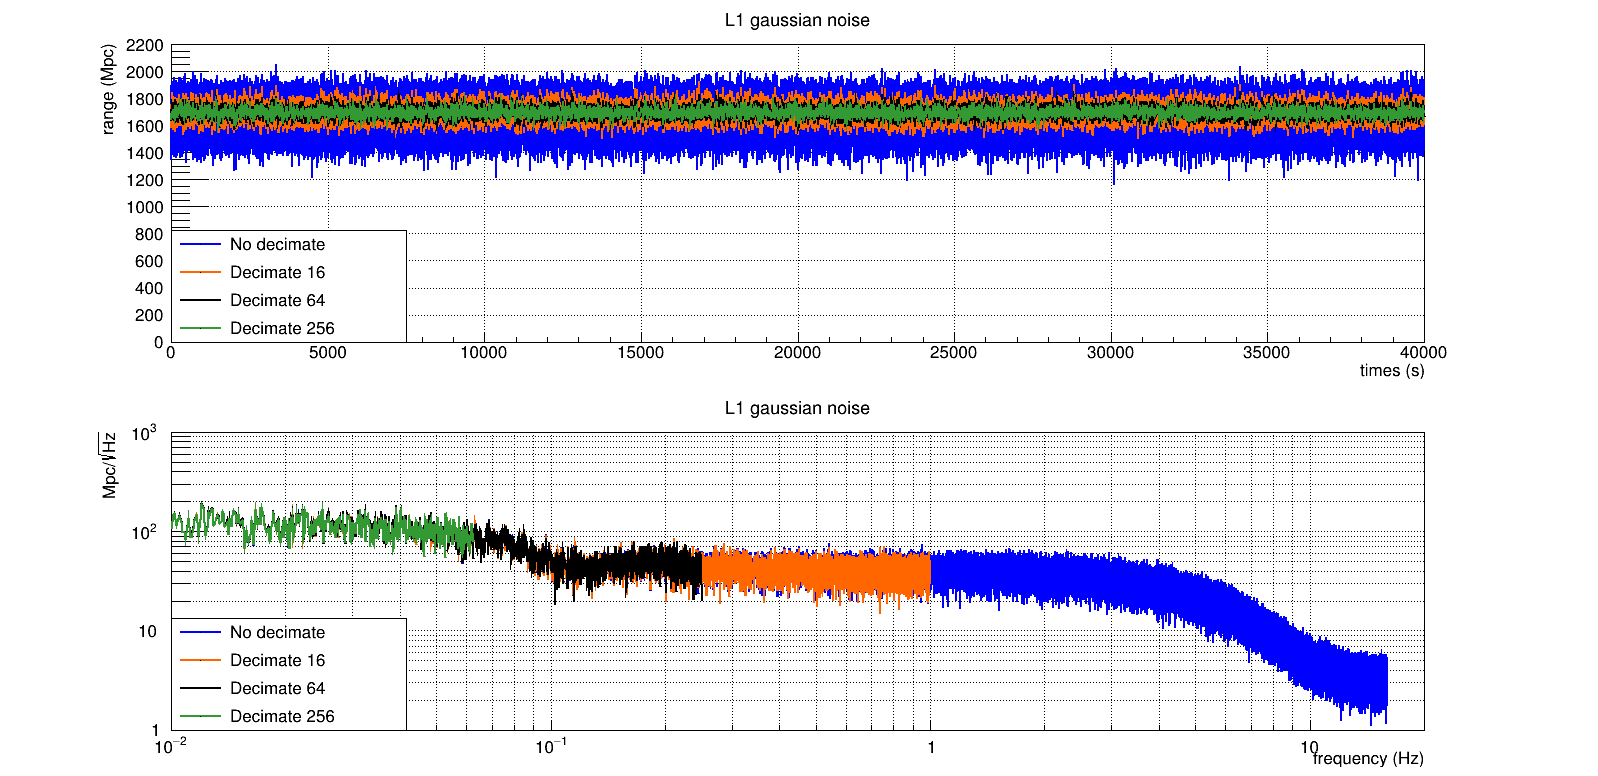
\includegraphics[width=\linewidth]{sectionBadTriggers/PSD/Range/range_PSD/cGaus_L1_BBH.png}
%   \captionof{figure}{BBH range in the time and frequency domain, computed from 10Hz on Gaussian noise}
%   \label{fig:rangeGaus_BBH_10}
% \end{figure}
% % 
% \begin{figure}[H]
%   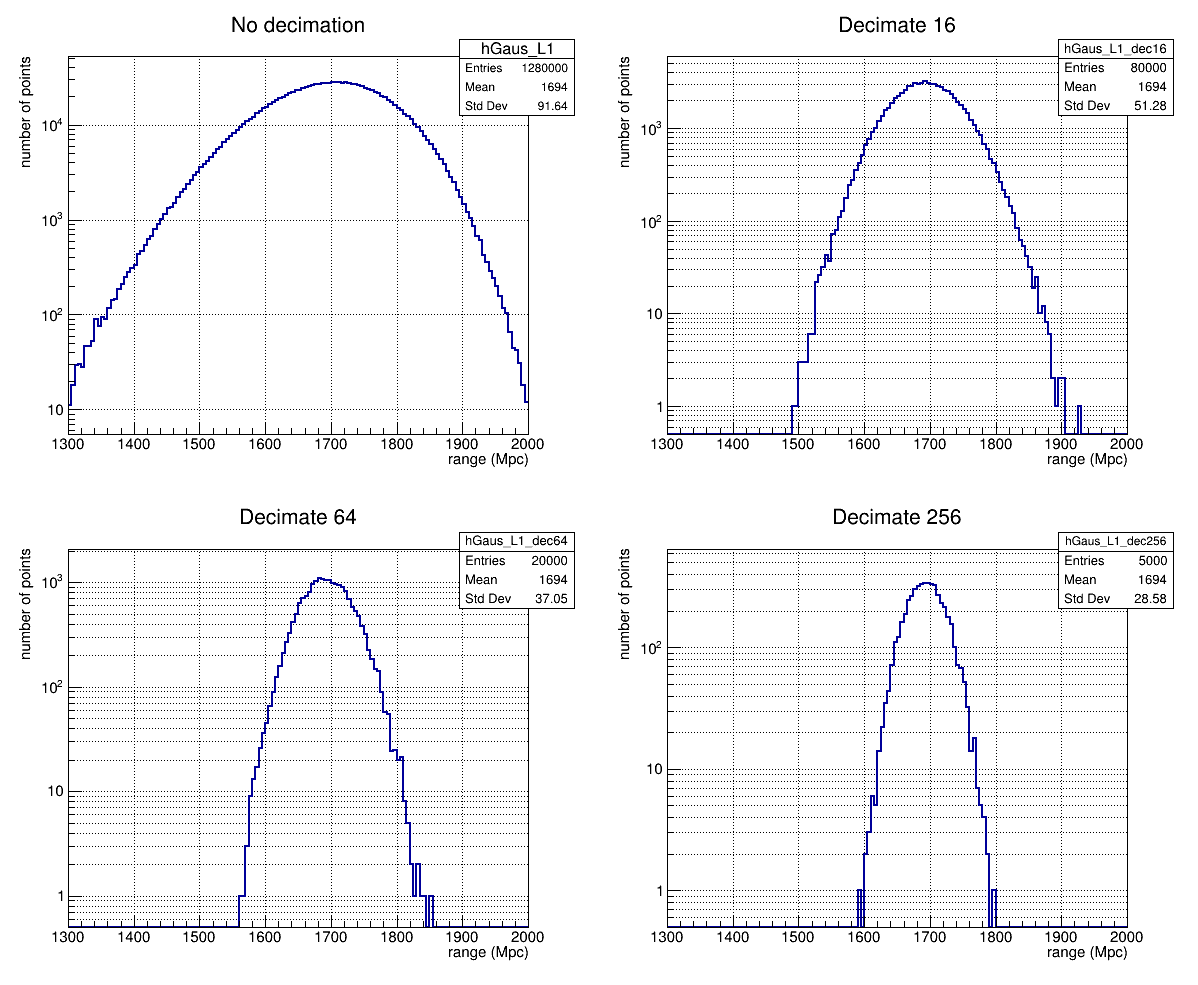
\includegraphics[width=\linewidth]{sectionBadTriggers/PSD/Range/range_PSD/c1DGaus_L1_BBH.png}
%   \captionof{figure}{1D projection of the BBH range in time domain computed from 10Hz on Gaussian noise}
%   \label{fig:rangeGaus_BBH_10_1D}
% \end{figure}
% % 
% \begin{figure}[H]
%   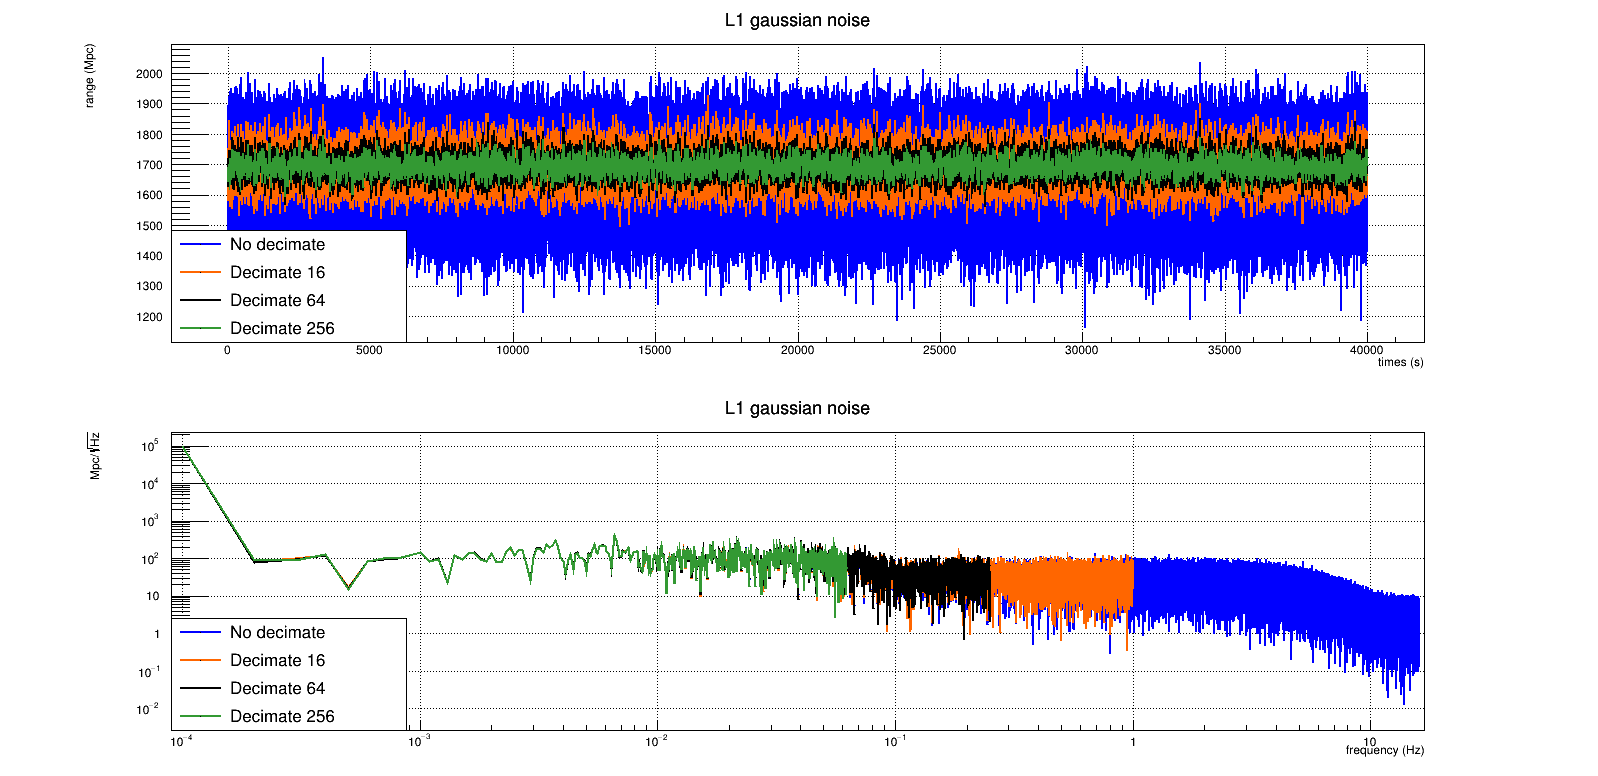
\includegraphics[width=\linewidth]{sectionBadTriggers/PSD/Range/range_PSD/cGaus_L1_BBH_20Hz.png}
%   \captionof{figure}{BBH range in the time and frequency domain, computed from 20Hz on Gaussian noise}
%   \label{fig:rangeGaus_BBH_20}
% \end{figure}
% % 
% \begin{figure}[H]
%   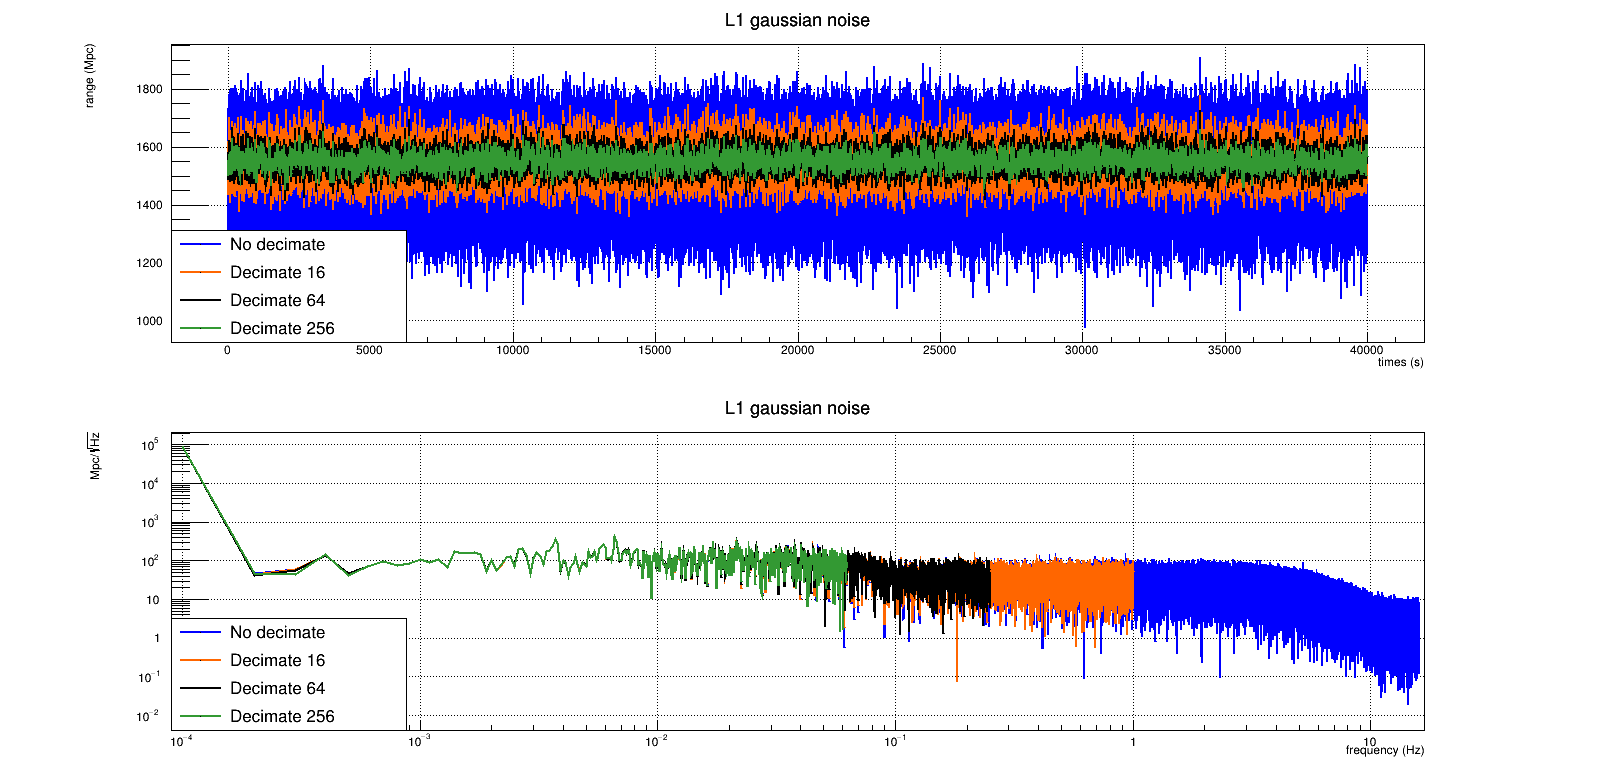
\includegraphics[width=\linewidth]{sectionBadTriggers/PSD/Range/range_PSD/cGaus_L1_BBH_50Hz.png}
%   \captionof{figure}{BBH range in the time and frequency domain, computed from 50Hz on Gaussian noise}
%   \label{fig:rangeGaus_BBH_50}
% \end{figure}
